\section{Valuing new goods in characteristics space}\label{sec:10-charspace}

The methods of \cref{sec:10-virtual,sec:10-functional} value a new good in product space. They estimate the
demand curve of the good itself and integrate under it up to the virtual price. This section treats a product
as a bundle of characteristics instead, in the tradition of \citet{Lancaster1966,Lancaster1971} and
\citet{McFadden1981}. The change of viewpoint has three consequences for welfare measurement. First, a
characteristics model can predict the demand for a product that has never been sold. Second, discrete-choice
models deliver consumer surplus in closed form, so the value of a change in the choice set is a simple function
of estimated parameters. Third, the functional forms that make these models tractable carry strong implicit
assumptions about the value of variety. Most of the section makes those assumptions explicit and compares the
models that impose them with models that do not.

Throughout the section a market has inside products $j = 1,\dots,J$ and an outside good $j = 0$. Consumer $i$
has income $y_i$, and we use the notation of \cref{ch:logit,ch:blp} for mean utilities $\delta_j$, deviations
$\mu_{ij}$ and idiosyncratic shocks $\epsilon_{ij}$. Where we discuss \citet{Trajtenberg1989}, we write
$\mathcal{W}(S)$ for his surplus function over a choice set $S$. We also write $z_j$ for the vector of
characteristics of product $j$ and $\tilde p_j$ for its residual price relative to a hedonic price function.

\subsection{Predicting demand for products that have never been sold}\label{sec:10-cs-predict}

A new product is a new point in characteristics space. Suppose a demand model has been estimated on existing
products, and the new product combines characteristics that lie within the range spanned by them. The estimated
tastes for characteristics then predict the new product's market share at any price, and the equilibrium pricing
conditions of \cref{ch:diffprod} predict its price. A product-space system cannot do this, because its
parameters are indexed by products and the new product has none \citep[pp.~1--2]{BerryPakes2007}. Berry and
Pakes add a second advantage. The number of parameters of a characteristics model does not grow with the number
of products. A log-linear product-space system for $J$ products needs a number of parameters of the order of $J^2$. \Citet{BerryLevinsohnPakes2004} use this property to simulate the demand for products before launch.

The same property disciplines the retrospective valuation of products that already exist. We never observe
demand at prices high enough to reveal the reservation prices of most buyers. Every estimate of the surplus
from a product therefore extrapolates beyond the data \citep[p.~2]{BerryPakes2007}. A product-space system extrapolates the
product's own demand curve to high prices, as in \cref{sec:10-functional}. A characteristics model uses slightly
more information. It borrows the price variation of other products with similar characteristics, although the
functional form still governs the extrapolation.

The approach has three limits. The first is an \emph{entirely new characteristic}, one that no existing product
possesses. Tastes for it cannot be learned from existing products. An electric car, for example, has a range, a
charging time and no fuel cost, so its demand cannot be inferred from the demand for gasoline cars alone. The
second limit is attributes that resist measurement, such as the plot of a book or the style of a film. When the
relevant attributes cannot be coded as a short vector $x_j$, the approach loses its dimension reduction. The third
limit is the \emph{radical innovation}, a product that opens a new product class. \Citet[pp.~10--11]{Trajtenberg1985}\footnote{We cite
\citet{Trajtenberg1989} through its working-paper version \citep{Trajtenberg1985}, the text available to us. Page,
table and equation numbers for this study refer to the working paper, as explained in \cref{sec:10-trajtenberg}.}
argues that a welfare comparison requires a choice set and a surplus function defined before the innovation, and
a radical innovation offers neither. He quotes \citet[p.~28]{Kuznets1962} on the point. For Kuznets, a rough
estimate of the value of a new product ``seems to be possible only if the new product can be treated as a substitute
for the old one.''
Trajtenberg's response is to measure the improvements that follow the first commercial product, and to infer the
value of the first product indirectly from the diffusion of the innovation (\cref{sec:10-ct-diffusion}).

\Citet[p.~229]{Hausman1997} pushes the first two limits further, as \cref{sec:10-hausman-ces} reports. He
describes each cereal brand by its own indicator variable and doubts that a brand such as Apple-Cinnamon Cheerios
can be described by its attributes. For him the natural measure of distance between products is the cross-price
elasticity. \Citet[p.~238, n.~3]{Bresnahan1997} reads the characteristics approach more favorably. Trajtenberg used
an address model of differentiation. This led him to conjecture that a new good's distance from existing products
governs the slope of its demand curve $dd$, and hence its surplus (\cref{fig:10-dd-DD}). The propositions below
make this conjecture precise for the logit, the nested logit and the vertical model.

Finally, the characteristics models used in this section assume that each consumer buys one unit of one product.
Products can then only be substitutes. Complementarity between a new good and old goods requires a model of
bundles, which we study in \cref{sec:10-gentzkow}.

\subsection{Consumer surplus in random utility models}\label{sec:10-cs-welfare}

We begin with the welfare theory that all characteristics-based valuations share. The key assumption is that
income enters utility linearly, so that utility differences convert into money at a constant rate.

\begin{assumption}[Quasi-linear random utility]\label{ass:10-quasilinear}
Consumer $i$'s utility from product $j\in\{1,\dots,J\}$ and from the outside good are
\begin{equation}\label{eq:10-quasilinear}
u_{ij} = \alpha(y_i - p_j) + x_j\beta + \xi_j + \mu_{ij} + \epsilon_{ij},
\qquad
u_{i0} = \alpha y_i + \epsilon_{i0},
\end{equation}
with $\alpha > 0$. Write $\delta_j = x_j\beta - \alpha p_j + \xi_j$ and set $\delta_0 = \mu_{i0} = 0$. The shocks
$(\epsilon_{i0},\dots,\epsilon_{iJ})$ are independent of $(x,\xi,\mu_i)$, have a joint density and a finite mean.
In the logit case they are \iid\ type-I extreme value.
\end{assumption}

The term $\alpha y_i$ is common to all alternatives, so it does not affect choices. For a consumer with deviations
$\mu_i$, define the \emph{expected maximum utility} over a choice set $\mathcal{J}$ that contains the outside good,
\begin{equation}\label{eq:10-emax}
G_i(\mathcal{J}) = \E\left[\max_{j\in\mathcal{J}}\left(\delta_j + \mu_{ij} + \epsilon_{ij}\right)\right],
\end{equation}
where the expectation is over $\epsilon_i$.

\begin{lemma}[Compensating variation under quasi-linearity]\label{lem:10-cv-quasilinear}
Under \cref{ass:10-quasilinear}, let the choice set and prices change from $(\mathcal{J}^0,p^0)$ to
$(\mathcal{J}^1,p^1)$. Let $CV_i$ be the extra income that consumer $i$ would need, facing $(\mathcal{J}^0,p^0)$, to
reach the utility she attains at $(\mathcal{J}^1,p^1)$, as in \cref{def:10-cv}. For every realization of $\epsilon_i$,
\begin{equation}\label{eq:10-cv-draw}
CV_i = \frac{1}{\alpha}\left[\max_{j\in\mathcal{J}^1}\left(\delta^1_j + \mu_{ij} + \epsilon_{ij}\right)
- \max_{j\in\mathcal{J}^0}\left(\delta^0_j + \mu_{ij} + \epsilon_{ij}\right)\right],
\end{equation}
and the expected compensating variation is $\E[CV_i] = \frac{1}{\alpha}\left[G^1_i(\mathcal{J}^1) -
G^0_i(\mathcal{J}^0)\right]$, where $G^t_i$ uses the mean utilities $\delta^t$.
\end{lemma}

\begin{proof}
Adding $c$ to income before the change raises the utility of every alternative by $\alpha c$. The maximal utility
before the change, with the extra income, is therefore
\begin{equation*}
\alpha(y_i + c) + \max_{j\in\mathcal{J}^0}\left(\delta^0_j + \mu_{ij} + \epsilon_{ij}\right).
\end{equation*}
After the change, maximal utility is $\alpha y_i + \max_{j\in\mathcal{J}^1}(\delta^1_j + \mu_{ij} + \epsilon_{ij})$.
Setting the two equal and solving for $c$ gives \eqref{eq:10-cv-draw}. Taking expectations over $\epsilon_i$ gives
the second statement.
\end{proof}

Because income effects are absent, the compensating and equivalent variations coincide here. Under quasi-linearity
we therefore call $\frac{1}{\alpha}G_i(\mathcal{J})$, up to a constant, the \emph{expected consumer surplus}
$CS_i(\mathcal{J})$. This is the measure of \citet{SmallRosen1981} and \citet{McFadden1981}. The next lemma shows
that it is the integral under the demand curves, so it is the discrete-choice counterpart of the Hicksian area in
\cref{prop:10-cv-newgood}.

\begin{lemma}[Williams-Daly-Zachary, \citealp{McFadden1981}]\label{lem:10-wdz}
Let $\epsilon = (\epsilon_0,\dots,\epsilon_J)$ have a joint density and a finite mean, and let
$G(\delta) = \E[\max_k(\delta_k + \epsilon_k)]$. Then $G$ is differentiable and
$\frac{\partial G}{\partial \delta_j} = \Pr\left(j = \argmax_k(\delta_k + \epsilon_k)\right)$ for every $j$.
\end{lemma}

The lemma restates part (ii) of \cref{thm:06-wdz} with $V = \delta$. The proof there bounds the difference
quotient of the maximum by one and applies dominated convergence.

Two consequences follow. Since $\delta_j$ contains $-\alpha p_j$, the chain rule gives
\begin{equation}\label{eq:10-roy}
\frac{\partial CS_i}{\partial p_j} = \frac{1}{\alpha}\,\frac{\partial G_i}{\partial \delta_j}\,(-\alpha) = -s_{ij},
\end{equation}
where $s_{ij}$ is consumer $i$'s choice probability. This is Roy's identity for discrete choice, and
\citet[p.~19, n.~18]{Trajtenberg1985} uses it to verify his surplus function. Consumer surplus is thus the area under
the probabilistic demand curves, and the change in $CS_i$ from raising $p_n$ to infinity is the area under
product $n$'s demand curve. The second consequence is a closed form in the logit case.

\begin{lemma}[Log-sum formula]\label{lem:10-logsum}
If $\epsilon_0,\dots,\epsilon_J$ are \iid\ type-I extreme value, then $\max_k(\delta_k + \epsilon_k)$ is
type-I extreme value with location $\ln\sum_{k=0}^{J} e^{\delta_k}$, and
\begin{equation}\label{eq:10-logsum}
\E\left[\max_k(\delta_k + \epsilon_k)\right] = \ln\sum_{k=0}^{J} e^{\delta_k} + \gamma_E,
\end{equation}
where $\gamma_E \approx 0.5772$ is Euler's constant.
\end{lemma}

The first statement is the max-stability of the Gumbel distribution (\cref{lem:06-maxstable}). The second is
\cref{prop:06-logsum} with $V_{ik} = \delta_k$ and $\sigma_\epsilon = 1$.

With $\delta_0 = 0$, the logit consumer surplus is therefore
\begin{equation}\label{eq:10-logit-cs}
CS = \frac{1}{\alpha}\ln\left(1 + \sum_{k=1}^{J}e^{\delta_k}\right) + C,
\end{equation}
where $C$ collects income and $\gamma_E$ and does not depend on the choice set. \Cref{sec:06-tiev} derives the
extreme value algebra and the logit shares. Trajtenberg's surplus function is the
same object, $\mathcal{W}(S) = \frac{1}{\alpha}\ln\sum_{j\in S}e^{V_j}$, written for a choice set $S$ of scanners
without an outside good. We now use \eqref{eq:10-logit-cs} to value an introduction.

\begin{proposition}[Value of a new product in the logit model]\label{prop:10-logit-newgood}
In the logit model, add product $n$ with mean utility $\delta_n$ to a market with products $1,\dots,J$, holding
the other mean utilities fixed. Per consumer, consumer surplus rises by
\begin{equation}\label{eq:10-logit-newgood}
\Delta CS = \frac{1}{\alpha}\ln\left(1 + \frac{e^{\delta_n}}{1 + \sum_{k=1}^{J}e^{\delta_k}}\right)
= -\frac{1}{\alpha}\ln(1 - s_n),
\end{equation}
where $s_n$ is the market share of product $n$ after the introduction.
\end{proposition}

\begin{proof}
The introduction reverses the removal of $n$ from the post-introduction market. By \eqref{eq:07-removal-logit} in
\cref{cor:07-removal}, that removal changes surplus by $\frac{1}{\alpha}\ln(1 - s_n)$, with $s_n$ the share before
the removal, which is the share after the introduction. The introduction therefore raises surplus by
$-\frac{1}{\alpha}\ln(1 - s_n)$. For the first expression, let $A_0 = 1 + \sum_{k=1}^{J}e^{\delta_k}$ and
$A_1 = A_0 + e^{\delta_n}$. Then $s_n = \frac{e^{\delta_n}}{A_1}$, so $1 - s_n = \frac{A_0}{A_1}$ and
$-\ln(1 - s_n) = \ln\frac{A_1}{A_0} = \ln\big(1 + \frac{e^{\delta_n}}{A_0}\big)$.
\end{proof}

The proposition has a strong implication. The value of a new product depends only on its share and on the
price coefficient. Two products with the same share are worth the same, whether one is a novel design and the
other a near copy of an existing product. The characteristics of the new product matter only through the share
they produce. The CES variety index of \cref{cor:10-ces-newgood} has the same property, since it depends only on
the new good's expenditure share and the elasticity of substitution. \Cref{rem:10-ces-logit} explains why the
two results are close relatives: the CES demand system is the aggregate demand of logit consumers
\citep{AndersonDePalmaThisse1992}.

The proposition also bounds the gain of the average buyer of the new product. For $s \in (0,1)$ we have
$s \le -\ln(1 - s) \le \frac{s}{1-s}$, by the series $-\ln(1-s) = \sum_{m\ge1}\frac{s^m}{m}$. Dividing
\eqref{eq:10-logit-newgood} by $s_n$ therefore gives
\begin{equation}\label{eq:10-logit-perbuyer}
\frac{1}{\alpha} \le \frac{\Delta CS}{s_n} \le \frac{1}{\alpha(1 - s_n)} .
\end{equation}
The upper bound is the markup of a single-product logit firm (\cref{prop:10-clones} below). So in the logit
model the average buyer of a new product gains at least $\frac{1}{\alpha}$ dollars, however close the product is
to existing ones. She gains roughly as much as the firm earns per unit sold. For a small share, $\Delta CS \approx
\frac{s_n}{\alpha}$. The market-level gain is $M\,\Delta CS$ for a market of size $M$. If the introduction also
changes rivals' prices, as in \cref{prop:10-logit-rivals}, the formula measures the variety effect at the new
prices, and the price effect must be added.

Nesting relaxes the result in the direction that \citet{Bresnahan1997} and Trajtenberg anticipate. Partition the
inside products into nests $g = 1,\dots,G$ and place the outside good in its own nest. In the nested logit of
\cref{ch:logit}, with nesting parameter $\sigma\in[0,1)$, define the inclusive value sums
$D_g = \sum_{j\in g}e^{\frac{\delta_j}{1-\sigma}}$. Shares and consumer surplus are
\begin{equation}\label{eq:10-nl-shares}
s_{j|g} = \frac{e^{\frac{\delta_j}{1-\sigma}}}{D_g},
\qquad
s_g = \frac{D_g^{1-\sigma}}{1 + \sum_{h=1}^{G}D_h^{1-\sigma}},
\qquad
CS = \frac{1}{\alpha}\ln\left(1 + \sum_{h=1}^{G}D_h^{1-\sigma}\right) + C .
\end{equation}

\begin{proposition}[Value of a new product in the nested logit model]\label{prop:10-nested-newgood}
In the nested logit model \eqref{eq:10-nl-shares}, add product $n$ to nest $g$, holding the other mean utilities
fixed. Per consumer, consumer surplus rises by
\begin{equation}\label{eq:10-nested-newgood}
\Delta CS = -\frac{1}{\alpha}\ln\left[1 - s_g + s_g\left(1 - s_{n|g}\right)^{1-\sigma}\right],
\end{equation}
where $s_g$ is the share of nest $g$ and $s_{n|g}$ the within-nest share of product $n$, both after the
introduction. For fixed post-introduction shares, $\Delta CS$ equals the logit value $-\frac{1}{\alpha}\ln(1-s_n)$
at $\sigma = 0$, falls strictly as $\sigma$ rises, and tends to zero as $\sigma\to 1$.
\end{proposition}

\begin{proof}
Let primes denote post-introduction values. Only nest $g$ changes:
$D_g' = D_g + e^{\frac{\delta_n}{1-\sigma}}$. Since $s_{n|g} = \frac{e^{\frac{\delta_n}{1-\sigma}}}{D_g'}$, we have
\begin{equation*}
D_g = D_g' - e^{\frac{\delta_n}{1-\sigma}} = D_g'\left(1 - s_{n|g}\right).
\end{equation*}
Write $A' = 1 + \sum_h D_h'^{1-\sigma}$ and $A = 1 + \sum_h D_h^{1-\sigma}$. Then
\begin{equation*}
A = A' - D_g'^{1-\sigma} + D_g^{1-\sigma} = A' - D_g'^{1-\sigma} + D_g'^{1-\sigma}\left(1 - s_{n|g}\right)^{1-\sigma}.
\end{equation*}
Dividing by $A'$ and using $s_g = \frac{D_g'^{1-\sigma}}{A'}$ gives
\begin{equation*}
\frac{A}{A'} = 1 - s_g + s_g\left(1 - s_{n|g}\right)^{1-\sigma}.
\end{equation*}
Since $\Delta CS = \frac{1}{\alpha}\ln\frac{A'}{A} = -\frac{1}{\alpha}\ln\frac{A}{A'}$, \eqref{eq:10-nested-newgood}
follows. At $\sigma = 0$ the bracket is $1 - s_g s_{n|g} = 1 - s_n$. Because $0 < 1 - s_{n|g} < 1$, the term
$(1 - s_{n|g})^{1-\sigma}$ rises strictly with $\sigma$ and tends to 1. The bracket therefore rises toward 1, and
$\Delta CS$ falls toward zero.
\end{proof}

The nesting parameter measures how close the new product is to the other members of its nest. At $\sigma = 0$
every product is an equally distant substitute and the logit value applies. As $\sigma \to 1$ the products within
a nest become perfect substitutes, and a new member of a crowded nest adds nothing. This is Bresnahan's point about
the slope of $dd$ in discrete-choice form. A new product that steals its share from close substitutes has a flat
demand curve and little surplus. With $s_g = 0.3$ and $s_{n|g} = 0.1$, for example, the gain in units of
$\frac{1}{\alpha}$ is 0.0305 at $\sigma = 0$, 0.0155 at $\sigma = 0.5$ and 0.0032 at $\sigma = 0.9$.

Trajtenberg writes the nested logit in a different but equivalent way, which matters for reading his estimates.
His within-nest index is $V_j = \frac{\delta_j}{1-\sigma}$, so the within-nest shares are $s_{j|g} =
\frac{e^{V_j}}{\sum_{k\in g}e^{V_k}}$. His nest-level parameter is $\lambda = 1 - \sigma$, and the inclusive value
of nest $g$ is $W_g = \ln\sum_{k\in g}e^{V_k}$. The nest shares are $s_g = \frac{e^{a_g + \lambda
W_g}}{\sum_h e^{a_h + \lambda W_h}}$, where we have added nest constants $a_g$ that his specification sets to
zero. In a sequential estimator, the coefficients inside $V_j$ are estimated in a first stage and then held fixed.
Let $\alpha_V = \frac{\alpha}{\lambda}$ denote the price coefficient inside $V_j$. Differentiating $\ln s_j =
V_j - W_g + a_g + \lambda W_g - \ln\sum_h e^{a_h+\lambda W_h}$ gives, for $j\in g$,
\begin{equation}\label{eq:10-nl-semi}
\frac{\partial\ln s_j}{\partial V_k} =
\begin{cases}
-s_{k|g}\left[1 - \lambda(1 - s_g)\right], & k\in g,\ k\ne j,\\[2pt]
-\lambda\, s_k, & k\in h \ne g .
\end{cases}
\end{equation}
Holding the $V$'s fixed, $\lambda\to0$ drives the cross-nest effects to zero while the within-nest effects stay
bounded away from zero. In this parameterization a small $\lambda$ therefore means that the nests are separate
markets, which is the reading \citet[p.~43, n.~42]{Trajtenberg1985} gives it. With $\delta_j$ held fixed instead,
$\sigma\to1$ makes products within a nest perfect substitutes. The two readings differ only in what is held
fixed. The money value of a change in the inclusive values has a simple limit.

\begin{corollary}[Separate markets]\label{cor:10-separate-markets}
In the parameterization above, consumer surplus is $CS = \frac{1}{\lambda\alpha_V}\ln\sum_h e^{a_h + \lambda W_h}
+ C$. Let the inclusive values change from $W^0_h$ to $W^1_h$, and let $s^0_h = \frac{e^{a_h}}{\sum_m e^{a_m}}$.
Holding $\alpha_V$, the $a_h$ and the $W$'s fixed, as $\lambda\to 0$
\begin{equation}\label{eq:10-separate-markets}
\Delta CS \;\to\; \sum_h s^0_h\,\frac{W^1_h - W^0_h}{\alpha_V}.
\end{equation}
\end{corollary}

\begin{proof}
In the units of $\delta$, the marginal utility of income is $\alpha = \lambda\alpha_V$, and nest-level consumer
surplus is $\frac{1}{\alpha}\ln\sum_h e^{a_h + \lambda W_h}$ by the nested version of \cref{lem:10-logsum}. Define
$f(\lambda) = \ln\sum_h e^{a_h + \lambda W^1_h} - \ln\sum_h e^{a_h + \lambda W^0_h}$, so that $\Delta CS =
\frac{f(\lambda)}{\lambda\alpha_V}$. Then $f(0) = 0$ and
\begin{equation*}
f'(0) = \sum_h \frac{e^{a_h}}{\sum_m e^{a_m}}\,W^1_h - \sum_h \frac{e^{a_h}}{\sum_m e^{a_m}}\,W^0_h
= \sum_h s^0_h\left(W^1_h - W^0_h\right).
\end{equation*}
By l'H\^opital's rule, $\frac{f(\lambda)}{\lambda}\to f'(0)$, which gives \eqref{eq:10-separate-markets}.
\end{proof}

When the nests are separate markets, the nest shares no longer respond to the products, and the value of a change
is the share-weighted average of the within-nest log-sum changes. This is exactly how Trajtenberg aggregates the
gains in head and body scanners (\cref{sec:10-ct-welfare}).

\casehead{Random coefficients and income effects} With random coefficients the logit formula holds consumer by
consumer. Conditional on $(D_i,\nu_i)$, the logit form gives $CS_i = \frac{1}{\alpha_i}\ln(1 + \sum_k
e^{\delta_k + \mu_{ik}})$, and the market measure integrates this over the distribution of $(D_i,\nu_i)$, as in
\cref{ch:blp}. Income effects break the log-sum formula. \Citet{Petrin2002} uses $\alpha_i\ln(y_i - p_j)$ in place
of $\alpha(y_i - p_j)$, so the marginal utility of income varies with $y_i - p_j$. Let the introduction change the
choice set from $\mathcal{J}^0$ at prices $p^0$ to $\mathcal{J}^1$ at prices $p^1$. With the standard of living
after the introduction as the reference, as in \cref{def:10-cv}, the compensating variation of consumer $i$ solves
\begin{equation}\label{eq:10-cv-income}
\max_{j\in\mathcal{J}^0}u_{ij}\left(y_i + CV_i,\, p^0\right) = \max_{j\in\mathcal{J}^1}u_{ij}\left(y_i,\, p^1\right).
\end{equation}
It depends on the realized tastes, and its average over consumers is computed by simulation.
\begin{enumerate}
\item Draw $R$ simulated consumers. For each draw $r$, draw demographics $D_r$ from their empirical distribution,
taste shocks $\nu_r$, and an extreme value shock $\epsilon_{rj}$ for every product in $\mathcal{J}^0\cup
\mathcal{J}^1$. Use the same $\epsilon_{rj}$ for a product in both choice sets.
\item Compute the new maximal utility $\bar u_r = \max_{j\in\mathcal{J}^1}u_{rj}(y_r, p^1)$.
\item Find $CV_r$ by bisection on $c\mapsto\max_{j\in\mathcal{J}^0}u_{rj}(y_r + c, p^0) - \bar u_r$. This
function is continuous and strictly increasing in $c$, because utility rises with income for every product.
\item Average: $\widehat{\E[CV]} = \frac{1}{R}\sum_r CV_r$. Multiply by the market size for the total.
\end{enumerate}
For Petrin's logarithmic specification, step 3 even has a closed form, derived in \cref{sec:10-petrin-cv}. Other
income specifications need the root finder.
The average of the individual $CV_r$ differs in general from the income change that equates expected maximal
utilities. The two coincide under quasi-linearity, where $CV_r$ is linear in the utility difference.
\Cref{sec:10-petrin} applies this algorithm to the minivan and splits the result into a part due to observed
characteristics and a part due to the $\epsilon$'s.

\subsection{The idiosyncratic-taste problem}\label{sec:10-cs-epsilon}

Characteristics-based demand models fall into two families, and the difference between them drives the valuation
of new goods. Let $f(y_i,p_j)$ be a function with $f_y > 0$, $f_p < 0$ and $f_{py}\ge 0$, so that utility rises
with income, falls with price, and richer consumers are weakly less sensitive to price. The first family contains
the \emph{pure characteristics models},
\begin{equation}\label{eq:10-pure-classes}
U_{ij} = f(y_i,p_j) + \delta_j + \sum_k\beta_k x_{jk}\nu_{ik}
\qquad\text{or}\qquad
U_{ij} = f(y_i,p_j) + \delta_j - \sum_k\tau_k\left(x_{jk} - \nu_{ik}\right)^2 ,
\end{equation}
with $\tau_k > 0$. The first form is the pure hedonic model of \citet{BerryPakes2007}, in which $\nu_{ik}$ is a
taste for characteristic $k$. The second is the ideal-type model of \citet{AndersonDePalmaThisse1992}, in which
$\nu_{ik}$ is consumer $i$'s ideal level of characteristic $k$. The second family adds an idiosyncratic shock,
\begin{equation}\label{eq:10-blp-class}
U_{ij} = f(y_i,p_j) + \delta_j + \sum_k\beta_k x_{jk}\nu_{ik} + \epsilon_{ij},
\end{equation}
as in \citet{BerryLevinsohnPakes1995}. The shocks $\epsilon_{ij}$ are drawn independently for every product and
consumer. \Citet{BerryPakes2007} call the second family models with \emph{tastes for products}, because the
$\epsilon_{ij}$ act like a separate characteristic for each product. Following \citet{CaplinNalebuff1991}, one
can think of them as interactions between product-specific dummy variables and \iid\ tastes for each dummy.

The $\epsilon_{ij}$ mean that the product space can never be exhausted. Each new product arrives with a fresh set
of draws, so some consumers like it more than anything else on the market, whatever its observed characteristics.
The following proposition collects the implications for the logit.

\begin{proposition}[Clones in the logit model]\label{prop:10-clones}
In the logit model with $\delta_0 = 0$:
\begin{enumerate}[label=(\alph*)]
\item A \emph{clone} of product $j$, a new product with $\delta_n = \delta_j$, has a positive share and raises
consumer surplus by
\begin{equation}\label{eq:10-clone-gain}
\Delta CS = \frac{1}{\alpha}\ln\frac{1 + \sum_{k=1}^{J}e^{\delta_k} + e^{\delta_j}}{1 + \sum_{k=1}^{J}e^{\delta_k}}
= \frac{1}{\alpha}\ln\left(1 + s^0_j\right) > 0,
\end{equation}
where $s^0_j$ is product $j$'s share before the clone enters.
\item With $J$ identical products of mean utility $\delta$, $CS(J) = \frac{1}{\alpha}\ln(1 + Je^{\delta}) + C$,
and $CS(J) - \frac{1}{\alpha}\ln J \to \frac{\delta}{\alpha} + C$. Consumer surplus grows like
$\frac{1}{\alpha}\ln J$ without bound.
\item The equilibrium markup of a single-product firm satisfies $p_j - mc_j = \frac{1}{\alpha(1 - s_j)} \ge
\frac{1}{\alpha}$, however many products crowd the market.
\item Every product with finite $\delta_j$ has a positive share, so the model cannot rationalize a product with a
zero share.
\end{enumerate}
\end{proposition}

\begin{proof}
(a) Apply \eqref{eq:10-logit-cs} with $A_0 = 1 + \sum_k e^{\delta_k}$ and $A_1 = A_0 + e^{\delta_j}$. Then
$\frac{A_1}{A_0} = 1 + \frac{e^{\delta_j}}{A_0} = 1 + s^0_j$, which exceeds 1.
(b) With $J$ identical products, $\sum_k e^{\delta_k} = Je^{\delta}$. Then
\begin{equation*}
\frac{1}{\alpha}\ln(1 + Je^{\delta}) - \frac{1}{\alpha}\ln J = \frac{1}{\alpha}\ln\left(\frac{1}{J} + e^{\delta}\right)
\to \frac{\delta}{\alpha}.
\end{equation*}
(c) Firm $j$ maximizes $(p_j - mc_j)Ms_j$. The logit share derivative is $\frac{\partial s_j}{\partial p_j} =
-\alpha s_j(1 - s_j)$. The first-order condition is
\begin{equation*}
s_j - (p_j - mc_j)\,\alpha s_j(1 - s_j) = 0 ,
\end{equation*}
so $p_j - mc_j = \frac{1}{\alpha(1-s_j)}$. Since $0 < s_j < 1$, the markup exceeds $\frac{1}{\alpha}$.
(d) $s_j = \frac{e^{\delta_j}}{1 + \sum_k e^{\delta_k}} > 0$ for finite $\delta_j$.
\end{proof}

Each part is unrealistic in some markets. Part (a) is the red bus and blue bus problem of \cref{ch:logit} viewed
from the welfare side. Adding a blue bus identical to a red bus creates surplus in the logit, although nothing new
is offered. Part (b) says that proliferating near-identical brands raises welfare without bound. Part (c) says that
markups do not fall toward marginal cost as the product space fills. In a pure characteristics model, by contrast,
a clone is a perfect substitute for the original. At given prices it adds no variety value. If a rival sells it,
Bertrand competition drives both prices to cost, and consumers gain only through this price effect. If the
original's owner sells it, nothing changes. Part (d) is the mirror image of the others. The model must assign every
product a positive share, so it cannot use the information in products that sell nothing, and the inversion $\ln
s_j - \ln s_0 = \delta_j$ breaks down at zero shares. The same mechanism biases estimated markups and the
estimated welfare gains from new goods upward.

\citet[p.~18]{Trajtenberg1985} noticed the welfare side of this problem in 1985. He decomposed his surplus function
into a part due to observed utility and a part due to dispersion.

\begin{proposition}[Entropy decomposition]\label{prop:10-entropy}
Let $s_j = \frac{e^{V_j}}{\sum_k e^{V_k}}$ be logit choice probabilities over a finite choice set. Then
\begin{enumerate}[label=(\alph*)]
\item $\ln\sum_j e^{V_j} = \sum_j s_jV_j + \mathcal{H}(s)$, where $\mathcal{H}(s) = -\sum_j s_j\ln s_j$ is the
\emph{entropy} of the choice probabilities.
\item Conditional on choosing $j$, the maximal utility $V_j + \epsilon_j$ is type-I extreme value with location
$\ln\sum_k e^{V_k}$, for every $j$. Hence
\begin{equation*}
\E[\epsilon_j\mid j\text{ chosen}] = \gamma_E - \ln s_j
\qquad\text{and}\qquad
\mathcal{H}(s) = \sum_j s_j\left(\E[\epsilon_j\mid j\text{ chosen}] - \gamma_E\right).
\end{equation*}
\end{enumerate}
\end{proposition}

\begin{proof}
(a) For every $j$, $\ln s_j = V_j - \ln\sum_k e^{V_k}$, so $\ln\sum_k e^{V_k} = V_j - \ln s_j$. Multiply by $s_j$
and sum over $j$. Since $\sum_j s_j = 1$,
\begin{equation*}
\ln\sum_k e^{V_k} = \sum_j s_jV_j - \sum_j s_j\ln s_j .
\end{equation*}
(b) Let $f$ and $F$ be the type-I extreme value density and CDF, and let $A = \sum_k e^{V_k - V_j} =
\frac{1}{s_j}$. The event that $j$ is chosen and its utility is at most $m$ has probability
\begin{equation*}
\int_{-\infty}^{m - V_j} f(e)\prod_{k\ne j}F(V_j + e - V_k)\,de
= \int_{-\infty}^{m - V_j} e^{-e}\exp\left(-e^{-e}A\right)de .
\end{equation*}
Substitute $t = e^{-e}$, so $dt = -e^{-e}de$. The integral becomes
\begin{equation*}
\int_{e^{-(m - V_j)}}^{\infty}e^{-tA}\,dt = \frac{1}{A}\exp\left(-Ae^{-(m-V_j)}\right)
= s_j\exp\left(-e^{-\left(m - \ln\sum_k e^{V_k}\right)}\right).
\end{equation*}
Dividing by $\Pr(j\text{ chosen}) = s_j$ gives the conditional CDF, which does not depend on $j$. Its mean is
$\ln\sum_k e^{V_k} + \gamma_E$, so $\E[\epsilon_j\mid j] = \ln\sum_k e^{V_k} - V_j + \gamma_E = \gamma_E - \ln s_j$.
Multiplying by $s_j$ and summing gives the last identity.
\end{proof}

Part (a) is Trajtenberg's equation (11), and part (b) explains what the entropy term measures. The surplus
function equals the share-weighted observed utility $\sum_j s_jV_j$ plus the average idiosyncratic taste that
consumers realize on the products they choose. With $J$ identical products and no outside good,
$\sum_j s_jV_j = V$ and $\mathcal{H} = \ln J$, so the entire gain from proliferation is entropy. Trajtenberg
traces this taste for ``horizontal variety'' to the independence of irrelevant alternatives. He notes that it
rewards ``the proliferation of seemingly identical brands that may differ only in their unobserved (and thus
presumably less important) attributes'' \citep[p.~19]{Trajtenberg1985}. For some purposes he suggests netting
out the change in entropy and using $\Delta\mathcal{W} - \frac{1}{\alpha}\Delta\mathcal{H}$. The net measure is not
a clean fix. The entropy term also contains the real value of matching heterogeneous buyers to different
products, which a model with random coefficients would attribute to observed characteristics.

Whether the $\epsilon$'s should count at all depends on what they represent. Four interpretations are common. They
may be tastes for unobserved product attributes, measurement error, approximation error in the utility function,
or optimization mistakes. Only the first supports counting them as welfare. If consumers choose with errors, the
log-sum formula counts the errors as utility.

\casehead{How the value of variety grows} \Cref{fig:10-variety-value} compares the growth of consumer surplus as
identical or evenly spaced products are added, in four models. The two logit-based curves use
\cref{prop:10-clones,prop:10-nested-newgood}. In the nested logit, $J$ identical products in one nest give
$D^{1-\sigma} = J^{1-\sigma}e^{\delta}$, so $CS(J) = \frac{1}{\alpha}\ln(1 + J^{1-\sigma}e^{\delta})$. Surplus still
grows without bound, at the slower rate $\frac{1-\sigma}{\alpha}\ln J$.

The pure characteristics benchmark is a Hotelling line. Consumers are uniform on $[0,1]$ and each buys one unit
at a common price $p$ from the nearest of $J$ products. The products sit at $\ell_k = \frac{2k-1}{2J}$, and a
consumer at distance $d$ from her product loses $td^2$. Each product serves an interval of length $\frac{1}{J}$,
and within it the distance $d$ is uniform on $\left[0,\frac{1}{2J}\right]$. The average loss is therefore
\begin{equation*}
t\,\E[d^2] = t\cdot\frac{1}{3}\left(\frac{1}{2J}\right)^2 = \frac{t}{12J^2},
\end{equation*}
and with gross value $v$,
\begin{equation}\label{eq:10-hotelling-cs}
CS(J) = v - p - \frac{t}{12J^2},
\qquad
CS(J) - CS(1) = \frac{t}{12}\left(1 - \frac{1}{J^2}\right) \le \frac{t}{12}.
\end{equation}
The gain is bounded, and the increment from one more product, $\frac{t}{12}\left(\frac{1}{J^2} -
\frac{1}{(J+1)^2}\right)$, falls to zero like $\frac{t}{6J^3}$. Adding logit errors with scale $\mu$ to the same
line gives $CS(x) = \mu\ln\sum_k e^{-\frac{t(x - \ell_k)^2}{\mu}}$ for a consumer at $x$, up to a constant. The
sum divided by $J$ is a Riemann sum, so for large $J$ the sum is close to
$J\,I(x)$ with $I(x) = \int_0^1 e^{-\frac{t(x - \ell)^2}{\mu}}\,d\ell > 0$. Hence $CS(x) \approx \mu\ln J + \mu\ln I(x)$,
and the gain grows like $\mu\ln J$. The integral $I(x)$ is close to the whole-line value $\sqrt{\frac{\pi\mu}{t}}$
only when both $x$ and $1 - x$ are large relative to $\sqrt{\frac{\mu}{t}}$.

\begin{figure}[htbp]
\centering
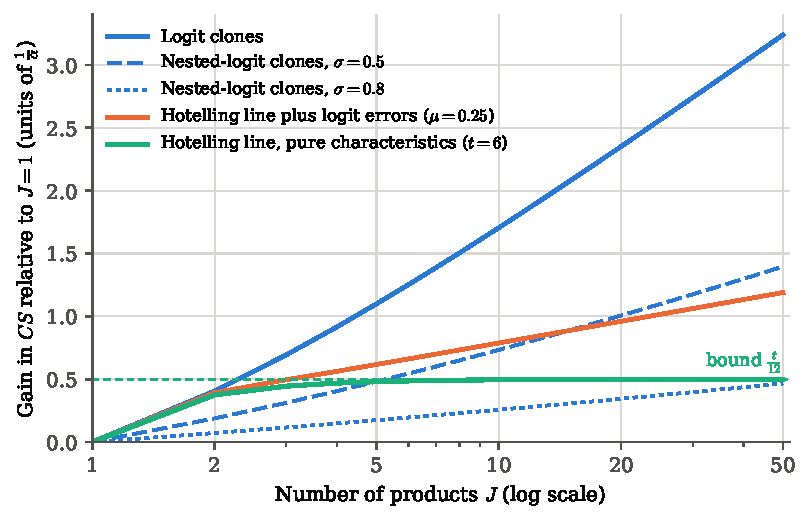
\includegraphics[width=0.88\textwidth]{figures/ch10/variety_value.pdf}
\caption{Gain in consumer surplus from adding products, relative to a market with one product, in units of
$\frac{1}{\alpha}$. The logit and nested-logit curves add identical products with $\delta = 0$ in the presence of
an outside good. The Hotelling curves place $J$ products evenly on a line with uniform consumers, quadratic
transport cost $t = 6$ and fixed equal prices. The orange curve adds logit errors with scale $\mu = 0.25$ to the
Hotelling model. At $J = 50$ the gains are 3.24 (logit), 1.40 and 0.47 (nested logit with $\sigma = 0.5$ and
$0.8$), 1.19 (Hotelling with errors) and 0.50 (pure Hotelling). Only the models with idiosyncratic errors grow
without bound. For the Hotelling curves we set $\alpha = 1$, so all curves are in the same units. Our
computations.}
\label{fig:10-variety-value}
\end{figure}

\Citet{AckerbergRysman2005} propose a correction within the logit family. It lets the contribution of the
idiosyncratic term depend on how crowded the product space is, so that additional products add less.

\subsection{Pure characteristics and vertical models}\label{sec:10-cs-pure}

\Citet{BerryPakes2007} develop the pure characteristics model for empirical work. Their utility is
\begin{equation}\label{eq:10-bp-utility}
u_{ij} = x_j\beta_i - \alpha_ip_j + \xi_j,
\qquad u_{i0} = 0,
\end{equation}
with random coefficients $\beta_{ik} = \beta_k + \sigma_k\nu_{ik}$ and $\alpha_i > 0$, after normalizing the
coefficient on the single unobserved characteristic $\xi_j$ to one. The model has no $\epsilon_{ij}$. They show
that the two families of models differ in two respects (pp.~2--3 and 6--7 of their text). With tastes for products,
substitution between products is limited and markups stay bounded away from zero as similar products are added.
Each consumer's utility also grows without bound as products are added, whatever their characteristics. In the
pure characteristics model, the gain from a new product is limited by a smooth function of its distance from
existing products. As the space fills, products become close substitutes, prices approach marginal cost, and the
increment in welfare from each new product declines to zero.

The $\epsilon$'s have practical advantages, which explain their popularity. They make choice probabilities
integrals with simple limits, and they keep every probability positive with smooth derivatives. They also allow the
share inversion that turns $\xi_j$ into a linear function of data and parameters
\citep{Berry1994,BerryLevinsohnPakes1995}.
Without them the share function has kinks and the inversion is no longer a contraction. Berry and Pakes therefore
propose to use the vertical model of \cref{ch:discrete} for the price coefficient, conditional on the other
coefficients, and a homotopy method to compute the mean utilities. A \emph{homotopy method} solves a hard system
of equations by deforming an easy system into it and following the solution path. They also study a ``modified BLP'' model in
which the logit term is scaled by $\frac{1}{\mu_\epsilon}$. The pure characteristics model is the limit as
$\mu_\epsilon\to\infty$.

\casehead{Welfare in a Monte Carlo experiment} The last experiment in \citet[Section 5.4]{BerryPakes2007} speaks to
new goods. The data come from a pure characteristics model with three markets, structured as successive years of
a market with improving characteristics. The number of products rises from 75 to 100 and then to 125. The
characteristics are patterned on the megahertz of personal computers in 1995--97 \citep{Pakes2003}, and prices for
given characteristics fall by roughly 30 percent a year. The welfare measure is the average gain per person, in
dollars, from moving from the year-one choice set to the year-three choice set. \Cref{tab:10-bp-welfare} reports
it.

\begin{table}[htbp]
\centering
\caption{Welfare gain from the year-one to the year-three choice set in the Berry-Pakes Monte Carlo}
\label{tab:10-bp-welfare}
\small
\begin{tabular}{@{}lr@{}}
\toprule
Method & Gain \\
\midrule
True (pure characteristics data-generating process) & 266.1 \\
Homotopy estimator of the pure characteristics model & 265.3 \\
Modified BLP, scale fixed at $\mu_\epsilon = 10$ & 270.0 \\
Modified BLP, scale $\mu_\epsilon$ estimated & 259.0 \\
Modified BLP, $\mu_\epsilon$ estimated, final homotopy contraction & 272.1 \\
\bottomrule
\end{tabular}

\smallskip
\begin{minipage}{0.86\linewidth}
\footnotesize Notes: Average per-person gain in dollars. One simulated data set with an average of 100 products per
market. The estimated scale in the fourth row is 0.934 with standard error 6.680, and the estimated constant in
mean utility is $-6.455$ against a true value of 2. Source: \citet{BerryPakes2007}, Tables 5 and 7.
\end{minipage}
\end{table}

All methods come within 3 percent of the truth. The modified BLP estimator with estimated scale does badly on
parameters and elasticities. For the lowest-priced product its own-price elasticity is $-1.8$ against a true
$-11.0$ \citep[Table 6]{BerryPakes2007}. Yet its welfare gain is close to the truth. Berry and Pakes explain why.
Because the contraction fits the shares exactly, the extra gain from the logit errors is offset by lower mean
utilities $\delta$, and the two roughly cancel. The estimated constant in $\delta$ falls below $-6$ to match the
small shares with a large logit error. The lesson is double-edged. Fitting shares exactly protects welfare
measures against part of the $\epsilon$ problem in this design, but it does so by distorting the parameters that
govern substitution.

\casehead{The hedonic approach} \Citet{BajariBenkard2005} take a different route to demand without
$\epsilon_{ij}$. Their method has two stages in the spirit of \citet{Rosen1974}. The first estimates a hedonic
price function $p_j = \mathbf{p}(x_j,\xi_j)$ that allows one unobserved characteristic and a non-additive form, and
recovers the $\xi_j$. They show that a hedonic price surface exists even with imperfect competition and finitely
many products. The second stage recovers tastes from each consumer's first-order conditions. At the chosen
product, the marginal utility of each continuous characteristic equals the marginal utility of money times the
slope of the price surface,
\begin{equation}\label{eq:10-bb-foc}
\frac{\partial u_i}{\partial x_{jk}} = \alpha_i\,\frac{\partial\mathbf{p}}{\partial x_{jk}} .
\end{equation}
With a continuum of products this inverts to each consumer's taste vector. With finitely many products the
revealed-preference conditions place each consumer's tastes in a set, which shrinks as the number of products
grows. The unobserved characteristic is essential. In their data on personal computers, 357 of 695 products are
dominated by another product that is better in every observed dimension and cheaper
\citep[p.~2]{BenkardBajari2004}.
They also note that the $\epsilon_{ij}$ amount to assuming an infinite-dimensional characteristics space, and that
logit-type demand curves typically are hyperbolic, approaching both axes. The hedonic model imposes no shape
beyond a downward slope, so the two families can predict quite different demand at prices outside the observed
range. That range is exactly where new-good valuations live.

\casehead{A vertical example} The vertical model of \cref{ch:discrete} makes the role of distance transparent.
Utility is $U_{ij} = \delta_j - \nu_ip_j$, with $\nu_i > 0$ distributed with continuous density $f$ on
$(0,\infty)$. A consumer's marginal utility of money is $\nu_i$, so a utility gain $\Delta U$ is worth
$\frac{\Delta U}{\nu_i}$ dollars to her. Products that sell are ordered by price and quality, and consumer $i$ buys
$j$ when $\nu_i$ lies between the cutoffs $c_{j,j+1} = \frac{\delta_{j+1}-\delta_j}{p_{j+1}-p_j}$ and $c_{j-1,j}$.

\begin{proposition}[Value of a new product in the vertical model]\label{prop:10-vertical-gain}
Let $j$ and $j+1$ be adjacent products with positive shares, $p_j < p_{j+1}$, and $c^* = c_{j,j+1} > 0$. Insert
product $n$ with $p_j < p_n < p_{j+1}$ and quality
\begin{equation}\label{eq:10-vertical-d}
\delta_n = \delta_j + c^*(p_n - p_j) + d ,
\end{equation}
so that $d$ is the vertical distance of the point $(p_n,\delta_n)$ above the chord joining $(p_j,\delta_j)$ and
$(p_{j+1},\delta_{j+1})$. Hold all other prices fixed, and take $d$ small enough that the new cutoffs stay inside
$(c_{j+1,j+2},\,c_{j-1,j})$.
\begin{enumerate}[label=(\alph*)]
\item If $d\le 0$, product $n$ sells nothing and creates no surplus.
\item If $d > 0$, exactly the consumers with $\nu\in(\nu_L,\nu_H)$ switch to $n$, where
\begin{equation*}
\nu_L = c^* - \frac{d}{p_{j+1} - p_n},
\qquad
\nu_H = c^* + \frac{d}{p_n - p_j}.
\end{equation*}
\item The money-metric gain of consumer $\nu$ is $g(\nu) = \frac{1}{\nu}\left[U_n(\nu) - \max\{U_j(\nu),
U_{j+1}(\nu)\}\right]^+$. It is positive on $(\nu_L,\nu_H)$ and equals $\frac{d}{c^*}$ at $\nu = c^*$.
\item The total gain $\mathcal{G} = \int g(\nu)f(\nu)\,d\nu$ satisfies the first expansion below. If in addition
$f(c^*) > 0$, the share $s_n$ is first order in $d$ and the gain per buyer satisfies the second,
\begin{equation}\label{eq:10-vertical-gain}
\mathcal{G} = \frac{f(c^*)}{2c^*}\,\frac{p_{j+1} - p_j}{(p_n - p_j)(p_{j+1} - p_n)}\,d^2 + o(d^2),
\qquad
\frac{\mathcal{G}}{s_n} = \frac{d}{2c^*} + o(d).
\end{equation}
\end{enumerate}
\end{proposition}

\begin{proof}
At $\nu = c^*$ the old products give equal utility, $U_j(c^*) = U_{j+1}(c^*)$. Using \eqref{eq:10-vertical-d},
\begin{equation*}
U_n(c^*) - U_j(c^*) = \delta_n - \delta_j - c^*(p_n - p_j) = d .
\end{equation*}
For $\nu > c^*$ the relevant rival is $j$, and $U_n(\nu) - U_j(\nu) = d - (\nu - c^*)(p_n - p_j)$. This difference
vanishes at $\nu_H$. For $\nu < c^*$ the rival is $j+1$, and $U_n(\nu) - U_{j+1}(\nu) = d + (c^* - \nu)(p_n -
p_{j+1})$, which vanishes at $\nu_L$. Both differences are linear in $\nu$ with peak $d$ at $c^*$.

(a) If $d \le 0$, $U_n(\nu) \le \max\{U_j(\nu),U_{j+1}(\nu)\}$ for every $\nu$, by the two linear expressions. No
consumer strictly prefers $n$.

(b) and (c) For $d > 0$, $n$ beats the better of $j$ and $j+1$ exactly on $(\nu_L,\nu_H)$. The bound on $d$
ensures that products other than $j$ and $j+1$ remain worse for these consumers. Dividing the utility gain by
$\nu$ gives $g(\nu)$, which equals $\frac{d}{c^*}$ at $c^*$.

(d) Let $h(\nu) = \nu g(\nu)$ denote the utility gain. It is a triangle with height $d$ and base $\nu_H - \nu_L$,
where
\begin{equation*}
\nu_H - \nu_L = d\left(\frac{1}{p_n - p_j} + \frac{1}{p_{j+1} - p_n}\right)
= d\,\frac{p_{j+1} - p_j}{(p_n - p_j)(p_{j+1} - p_n)} .
\end{equation*}
Its area is $\frac{1}{2}d(\nu_H - \nu_L)$. Since $\frac{f(\nu)}{\nu}$ is continuous at $c^* > 0$ and the interval
shrinks to $c^*$, $\frac{f(\nu)}{\nu} = \frac{f(c^*)}{c^*} + o(1)$ uniformly on it. Therefore
\begin{equation*}
\mathcal{G} = \int_{\nu_L}^{\nu_H}h(\nu)\frac{f(\nu)}{\nu}\,d\nu
= \left(\frac{f(c^*)}{c^*} + o(1)\right)\frac{d}{2}(\nu_H - \nu_L),
\end{equation*}
which is the first part of \eqref{eq:10-vertical-gain}. This step holds also when $f(c^*) = 0$, and the
coefficient on $d^2$ is then zero. The share is $s_n = F(\nu_H) - F(\nu_L) = (f(c^*) + o(1))(\nu_H - \nu_L)$.
When $f(c^*) > 0$, the factor $f(c^*) + o(1)$ is bounded away from zero for small $d$. Dividing the two
expressions then gives $\frac{\mathcal{G}}{s_n} = \frac{d}{2c^*} + o(d)$.
\end{proof}

The condition $f(c^*) > 0$ matters for the per-buyer formula. Take the density $f(\nu) = (\nu - 1)^2e^{-\nu}$,
old products $(p,\delta) = (1,2)$ and $(3,4)$, an outside utility of zero and the new product $(2,3+d)$. Then
$c^* = 1$ and $f(c^*) = 0$. Our computation gives $s_n = \frac{2e^{-1}d^3}{3} + o(d^3)$ and
$\mathcal{G} = \frac{e^{-1}d^4}{6} + o(d^4)$, so that $\frac{\mathcal{G}}{s_n} = \frac{d}{4} + o(d)$. This is half
the value $\frac{d}{2c^*} = \frac{d}{2}$ of \eqref{eq:10-vertical-gain}.

\Cref{fig:10-vertical-gain} draws the construction. When $f(c^*) > 0$, the gain is second order in the
distance $d$. The share of the new product is then first order in $d$, and the gain per buyer, $\frac{d}{2c^*}$,
vanishes as the new product approaches the chord. The quantity $\frac{d}{c^*}$ is the dollar value of the new product's quality premium at the margin
between its neighbors, and the average switcher gets half of it, as in any triangle. Compare
\eqref{eq:10-logit-perbuyer}. In the logit the gain per buyer is at least $\frac{1}{\alpha}$ for any product,
including a product on or below the chord. A numerical check with $f(\nu) = e^{-\nu}$ and the prices of
\cref{fig:10-vertical-gain} confirms \eqref{eq:10-vertical-gain}. The exact gain differs from the approximation by
1.7 percent at $d = 0.2$ and by 0.1 percent at $d = 0.05$.

\begin{figure}[htbp]
\centering
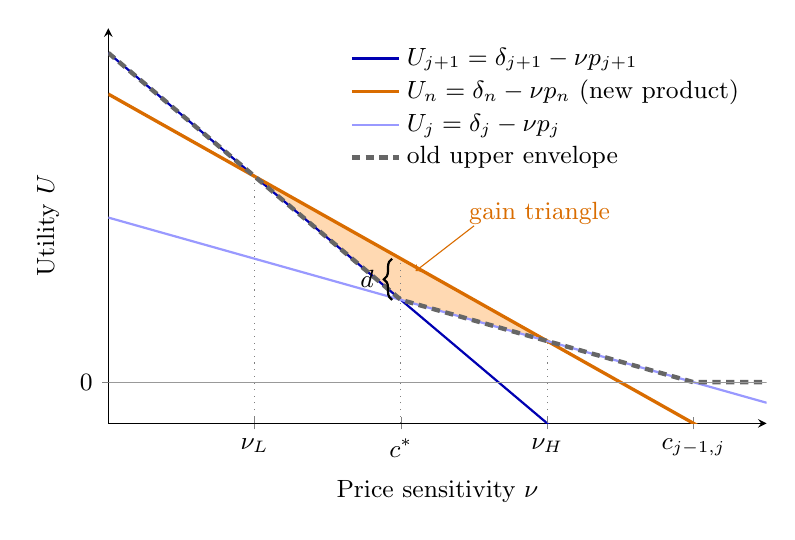
\begin{tikzpicture}
\begin{axis}[
  width=0.82\textwidth, height=6.6cm,
  xmin=0, xmax=2.25, ymin=-0.5, ymax=4.3,
  axis lines=left, clip=true,
  xlabel={Price sensitivity $\nu$}, ylabel={Utility $U$},
  xtick={0.5,1,1.5,2}, xticklabels={$\nu_L$,$c^*$,$\nu_H$,$c_{j-1,j}$},
  ytick={0}, yticklabels={$0$},
  every axis x label/.style={at={(axis description cs:0.5,-0.12)},anchor=north},
  every axis y label/.style={at={(axis description cs:-0.06,0.5)},rotate=90,anchor=south},
  tick label style={font=\small}, label style={font=\small},
  legend style={at={(0.98,0.98)}, anchor=north east, draw=none, fill=white, font=\small},
  legend cell align=left]
  \fill[orange!30] (axis cs:0.5,2.5) -- (axis cs:1,1) -- (axis cs:1.5,0.5) -- cycle;
  \addplot[blue!70!black, thick, domain=0:2.25, samples=2] {4 - 3*x};
  \addlegendentry{$U_{j+1} = \delta_{j+1} - \nu p_{j+1}$}
  \addplot[orange!85!black, very thick, domain=0:2.25, samples=2] {3.5 - 2*x};
  \addlegendentry{$U_n = \delta_n - \nu p_n$ (new product)}
  \addplot[blue!40, thick, domain=0:2.25, samples=2] {2 - x};
  \addlegendentry{$U_j = \delta_j - \nu p_j$}
  \addplot[black!60, densely dashed, line width=1.6pt] coordinates {(0,4) (1,1) (2,0) (2.25,0)};
  \addlegendentry{old upper envelope}
  \draw[black!50, dotted] (axis cs:0.5,-0.5) -- (axis cs:0.5,2.5);
  \draw[black!50, dotted] (axis cs:1,-0.5) -- (axis cs:1,1.5);
  \draw[black!50, dotted] (axis cs:1.5,-0.5) -- (axis cs:1.5,0.5);
  \draw[black!40] (axis cs:0,0) -- (axis cs:2.25,0);
  \draw[decorate, decoration={brace, amplitude=3pt}, thick] (axis cs:0.97,1.0) -- (axis cs:0.97,1.5)
     node[midway, left=3pt, font=\small] {$d$};
  \node[font=\small, orange!85!black, anchor=west] at (axis cs:1.2,2.05) {gain triangle};
  \draw[->, orange!85!black] (axis cs:1.25,1.9) -- (axis cs:1.05,1.35);
\end{axis}
\end{tikzpicture}
\caption{The vertical model with a product inserted between two neighbors. Each line is the utility $\delta - \nu p$
of one product as a function of price sensitivity $\nu$. The dashed line is the upper envelope before the
introduction, and the outside good gives utility zero. Product $n$ lies a distance $d$ above the chord joining its
neighbors and wins the consumers with $\nu\in(\nu_L,\nu_H)$. The shaded triangle is their utility gain, so the
welfare gain is of order $d^2$. The parameters are $(p_j,p_n,p_{j+1}) = (1,2,3)$ and $(\delta_j,\delta_n,\delta_{j+1}) =
(2,3.5,4)$, so $c^* = 1$ and $d = 0.5$.}
\label{fig:10-vertical-gain}
\end{figure}

\subsection{Hedonic methods, quality change and changing tastes}\label{sec:10-cs-hedonic}

Statistical agencies often handle new varieties with hedonic methods, and the vertical example shows what these
methods assume. A \emph{hedonic price function} $\mathbf{p}(z)$ relates the prices of products to their
characteristics $z$ \citep{Griliches1971,Rosen1974}. We write
\begin{equation}\label{eq:10-hedonic}
p_j = \mathbf{p}(z_j) + \tilde p_j ,
\end{equation}
where $\tilde p_j$ is the \emph{residual price}, the deviation of product $j$'s price from the surface. In Rosen's
model with a continuum of products, the hedonic function is an equilibrium locus. A consumer with utility
$\alpha[y - \mathbf{p}(z)] + \phi(z)$ chooses $z$ to satisfy $\mathbf{p}'(z) = \frac{\phi'(z)}{\alpha}$. A new
variety priced on the surface offers nothing that consumers could not already buy, so it adds no surplus. Hedonic
quality adjustment therefore treats a new variety as a perfect substitute for a combination of existing ones.
This is the flat curve $dd(-\infty)$ of \cref{fig:10-dd-DD}, which \citet[p.~238]{Bresnahan1997} identifies as an
understatement of the value of new goods. In the vertical model the chord between neighbors plays the role of the
hedonic surface. A product priced on it has $d = 0$ and adds nothing, while a product above it adds a gain of
order $d^2$. When the product space is sparse, the surface has wide gaps and the understatement can be large.

\casehead{Quality as repackaging} \citet[Section~10.3, pp.~262--266]{DeatonMuellbauer1980b} derive the most common
hedonic regression from a model in which quality repackages quantity. The varieties $j$ of a good are perfect
substitutes once each is weighted by a quality index $\zeta_j > 0$. Utility is
$v\bigl(h(\sum_j\zeta_jq_j),q_{\mathrm{other}}\bigr)$, where $q_{\mathrm{other}}$ collects the other goods (their
eq.~3.7). A consumer then buys only the varieties with the lowest price per unit of quality,
$\frac{p_{jt}}{\zeta_j}$. Suppose all consumers share the weights and every variety sells. The prices per unit of
quality must then be equal, $p_{jt} = \zeta_jP_t$, where $P_t$ is the price of a unit of quality in period $t$. With
$\ln\zeta_j = f(z_j)$, taking logs gives
\begin{equation}\label{eq:10-dm-hedonic}
  \ln p_{jt} = \ln P_t + f(z_j)
\end{equation}
(their eq.~3.8). A disturbance and a log-linear $f$ give the \emph{time-dummy hedonic regression}. It pools all periods
and adds a zero-one dummy for each period except a reference period (p.~263). The coefficients on the
period dummies estimate $\ln P_t$, a quality-corrected price index. A new variety priced on this surface sells
quality at the going price $P_t$, so it adds no surplus. Their Table~10.1 (p.~264) fits such a regression to 150
British used-car models, aged one to three years, from nine manufacturers in the late 1950s and the 1960s. A 1
percent increase in brake horsepower raises the price by 0.370 percent (standard error 0.023). The implied
quality-corrected price of cars was about 8 percent lower in 1969 than in 1958 (p.~263). The coefficients on miles
per gallon, $-0.064$ (0.041), and interior size, $-0.146$ (0.094), are negative and imprecise. Deaton and Muellbauer
suggest that, with length and width held fixed, a large interior may signal restricted luggage space (p.~264).
An $F$-test rejects a common price function across manufacturers. The statistic is 9, and 1.2 suffices to reject at
the 5 percent level (p.~265). Deaton and Muellbauer read this as evidence of \emph{market segmentation}, in which
products made for different types of consumers carry different shadow prices of characteristics (p.~259). A single
price surface ignores it. When consumers' weights differ, the surface is instead an envelope of their
\emph{bid functions}. A consumer's bid function gives the most she would pay for one unit of a variety with
characteristics $z$, at her utility level (pp.~265--266). The marginal condition
$\frac{\partial\ln\mathbf{p}(z)}{\partial z_k} = \frac{\partial\ln\zeta(z)}{\partial z_k}$ then holds for each
consumer at her chosen variety, as in \citet{Rosen1974} (eq.~3.10, pp.~265--266).

\casehead{Changing tastes: ex ante and ex post measures} Applications over long periods face a further problem.
If the estimated taste parameters change from year to year, the value of moving from choice set $S_t$ to $S_{t+1}$
depends on which year's tastes are used. Write $\mathcal{W}^t$ for the surplus function evaluated with the
parameters estimated for year $t$. \citet[pp.~56--58]{Trajtenberg1985} defines
\begin{equation}\label{eq:10-exante-expost}
\Delta\mathcal{W}^a = \mathcal{W}^t(S_{t+1}) - \mathcal{W}^t(S_t),
\qquad
\Delta\mathcal{W}^p = \mathcal{W}^{t+1}(S_{t+1}) - \mathcal{W}^{t+1}(S_t).
\end{equation}
The \emph{ex ante} measure $\Delta\mathcal{W}^a$ asks what a consumer with today's tastes would pay to face next
year's choice set. The \emph{ex post} measure $\Delta\mathcal{W}^p$ asks how much income could be taken from a
consumer with next year's tastes, leaving her indifferent between next year's and this year's sets. The
distinction resembles the one between compensating and equivalent variation, but it has a different source.
Compensating and equivalent variation hold tastes fixed and differ in the reference utility level, and they
coincide without income effects. Here utility is quasi-linear, and the ambiguity comes from the change in the taste
parameters themselves. The hybrid $\mathcal{W}^{t+1}(S_{t+1}) - \mathcal{W}^t(S_t)$ compares utilities under two
different preference structures, which is an interpersonal comparison and has no welfare meaning.

Trajtenberg expects the ex ante measure to exceed the ex post one. His argument is a \emph{dual inducement}
mechanism. Strong tastes for an attribute induce firms to improve that attribute, and the improvement then lowers
its marginal valuation next year. Judged by the original tastes, an improvement is therefore worth more. He also
considers a Divisia-like alternative that estimates adjacent years jointly. It yields a unique measure, but only by
suppressing the taste differences that create the problem.

\section{Case study: CT scanners (Trajtenberg 1989)}\label{sec:10-trajtenberg}

\citet{Trajtenberg1989} was the first study to measure a product innovation by the welfare it creates, using an
estimated discrete-choice demand system in characteristics space. The application is computed tomography (CT)
scanners in the United States from their introduction in 1973 to 1982. The paper is also an early study of how
innovation, diffusion and returns to research interact. The PDF available to us is the working-paper version
\citep{Trajtenberg1985}. All numbers below come from it, and page numbers refer to its typed pages. The
published version may number its tables differently, and some of its numbers may differ.
Trajtenberg indexes products by $i$ and characteristics by $j$. We index scanners by $j$ and characteristics by
$k$, consistent with the rest of the book.

\subsection{The question}\label{sec:10-ct-question}

The output of innovative activity does not come in countable units. Patent counts vary enormously in
significance, and sales of new products confound innovation with market size. Trajtenberg therefore argues that a
quantitative measure of innovation can only be defined in value terms
\citep[pp.~2--3]{Trajtenberg1985}. How much product innovation occurred in a field over a period is the
additional social surplus that the innovations generated. Other measures can at best serve as proxies.

A product is a pair $(z_j,p_j)$, with $z_j = (z_{j1},\dots,z_{jK})$ its characteristics and $p_j$ its price.
Trajtenberg writes $s_j$ for this pair, a symbol we keep for market shares.
The choice set in year $t$ is $S_t$, and product innovation is the change $S_t - S_{t-1}$. It includes improvements
in existing products, the addition of new ones and the exit of old ones. The magnitude of innovation is
\begin{equation}\label{eq:10-traj-dW}
\Delta\mathcal{W}_t = \mathcal{W}(S_t) - \mathcal{W}(S_{t-1}),
\end{equation}
for a surplus function $\mathcal{W}$ (equation 1 of the paper, p.~7). The measure includes the effect of price
changes. Trajtenberg defends this broad definition on practical grounds. With nonlinear surplus functions the
effects of characteristics and prices cannot be separated, and new products have no earlier price to compare with
(pp.~8--9).

What counts as a product innovation needs a definition, and Trajtenberg provides one through the nature of
characteristics (pp.~4--6).

\begin{definition}[Concatenable characteristics]\label{def:10-concatenable}
Let $x_j$ be the quantity of product $j$ that a consumer buys. Characteristic $k$ is \emph{concatenable} if the
amount of it available to the consumer is $z_{jk} = f^k(x_j)$ with $\frac{\partial z_{jk}}{\partial x_j} \ne 0$.
Examples are the protein in a food or the carrying capacity of vehicles. It is \emph{non-concatenable} if
$z_{jk} = g^k(\theta_j)$ for the product's natural unit $\theta_j$, with $\frac{\partial z_{jk}}{\partial x_j} = 0$
for $x_j > \theta_j$. Examples are the speed of a vehicle or the aperture of a camera.
\end{definition}

Product innovation requires at least one non-concatenable characteristic. Suppose all characteristics were
concatenable and linear in quantity. Then a change from $(z_j,p_j)$ to $(\kappa z_j,\kappa p_j)$ with
$\kappa > 1$ would leave the indirect utility unchanged, $V(z_j,p_j,y) = V(\kappa z_j,\kappa p_j,y)$. Buying $\kappa$ units of the old
product delivers the same bundle at the same cost. Such a change could not count as an innovation. A product
innovation therefore presupposes a quality dimension that can be changed only by switching products. CT scanners
satisfy this. Speed and image resolution are properties of the machine. Buying more machines does not change
them.

\casehead{Scope} The surplus function is in principle total surplus. Trajtenberg argues that profits pose no
special measurement problem beyond accounting, so the difficulty lies in consumer surplus. He measures the gains
that are not appropriated by the innovating firms and passed on to buyers (pp.~9--10). He states two limitations.
Radical innovations, which open new product classes, cannot be measured directly (\cref{sec:10-cs-predict}). The
measure also ignores spillovers to other product classes, so it is a lower bound on the social gain (pp.~11--12).
Trajtenberg proposes an indirect estimate of the gain from the first scanner, based on diffusion
(\cref{sec:10-ct-diffusion}).

The question matters for three reasons. Product innovation is a large part of technical change, and official
price and productivity statistics do not capture it (p.~1). Social returns to research cannot be computed without
a measure of benefits. And the interaction between innovation and diffusion cannot be studied without a measure of
innovation.

\subsection{Setting}\label{sec:10-ct-setting}

Research on computed tomography began in 1967 at the British electronics company EMI. The first operational
prototype was installed in a London hospital in 1971, and the first commercial system, the EMI Scanner, was
installed in the United States in June 1973 (p.~25). In 1974--77 nearly 20 firms entered. They ranged from
electronics companies (General Electric, Siemens, Hitachi, Philips) to pharmaceutical companies (Pfizer, Searle,
Syntex) and specialized firms (AS\&E, Elscint), and they competed mainly through product performance (p.~26).
Diffusion among U.S. hospitals was fast, the fifth fastest among twenty innovations for which diffusion studies
existed (p.~26, n.~23). Mounting concern about health-care costs led to Certificate of Need regulation, which
required approval for large hospital investments. Its full impact in 1978--79 produced a sharp downturn and the
exit of many firms, including EMI. The market then recovered and settled at 10--15 percent annual growth, with
General Electric holding about 50 percent of the U.S. market and some ten firms sharing the rest (p.~26). The two
pioneers of CT received the Nobel Prize in Medicine in 1979.

\casehead{Characteristics} A CT scanner takes cross-sectional images of the body. Trajtenberg measures three
performance characteristics (pp.~27--30). SPEED is the minimum scan time in seconds. The first scanner took five
minutes per scan, which restricted it to the brain, a motion-free organ. Scan times of twenty seconds and less
opened other organs, and the fastest systems of the early 1980s scanned in about one second. RESOL is spatial
resolution in millimeters, the size of the smallest object visible in high-contrast regions. Trajtenberg had
constructed a fuller image-quality index from experimental data, but it was unavailable for most of the roughly
50 systems marketed. RTIME is reconstruction time in seconds, the time the computer takes to produce the image. A
fourth attribute, gantry tilt, proved insignificant and was dropped. All three characteristics are defined so that
less is better. Scanners come in two types. \emph{Head scanners} can image only the brain, while \emph{body
scanners} can image almost any organ.

\subsection{Data}\label{sec:10-ct-data}

Trajtenberg assembled his own data bank, covering the period from the announcement of the innovation in 1972 to
1981, with some series extending to 1983 (pp.~30--32). It has four parts. The first gives the technical
characteristics and prices of all CT scanners marketed up to 1982, by year, which is the sequence of choice sets
$S_t$. The second records every installation in the United States, with the identity of the hospital or clinic,
the dates of order and installation, and the model bought. It has more than 2,000 observations, including
upgrades, and Trajtenberg estimates that it covers about 98 percent of U.S. installations up to July 1981. The
third describes the hospitals and the fourth the manufacturers, including their research and development spending
on CT. The main source is a questionnaire to all manufacturers, with follow-up contacts. Others are the radiology
and medical-physics literature, trade journals and consulting reports. Public sources include the Food and Drug
Administration, the Office of Technology Assessment, the Patent Office and the American Hospital Association, and
Trajtenberg also ran a telephone survey of hospitals.
All but two firms active in 1981 answered the questionnaire. The two were CGR and Philips, and Philips was excluded
for lack of reliable information. Little is lost, since it had sold fewer than twenty scanners in the United States by
1981.

A year in the data runs from November 1 of the previous year to October 31. Most new scanners are introduced at
the annual meeting of the Radiological Society of North America in November, so this \emph{radiological year}
matches the timing of choice sets. Data for 1981 cover only the first half of that year (p.~33, n.~28).
\Cref{tab:10-ct-data} reproduces Tables 1 and 2 of the paper.

\begin{table}[htbp]
\centering
\caption{CT scanners in the United States, 1973--1982}
\label{tab:10-ct-data}
\footnotesize
\setlength{\tabcolsep}{4.5pt}
\begin{tabular}{@{}lrrrrrrrr@{}}
\toprule
\multicolumn{9}{@{}l}{\textit{Panel A. Prices and average characteristics}} \\
& \multicolumn{2}{c}{Price (\$K)} & \multicolumn{2}{c}{SPEED (s)} & \multicolumn{2}{c}{RESOL (mm)} &
  \multicolumn{2}{c}{RTIME (s)} \\
\cmidrule(lr){2-3}\cmidrule(lr){4-5}\cmidrule(lr){6-7}\cmidrule(lr){8-9}
Year & Head & Body & Head & Body & Head & Body & Head & Body \\
\midrule
1973 & 310 & -- & 300 & -- & 3.1 & -- & 300 & -- \\
1974 & 370 & -- & 300 & -- & 1.7 & -- & 30 & -- \\
1975 & 379 & 365 & 285 & 195.0 & 1.8 & 1.6 & 20 & 8 \\
1976 & 374 & 471 & 105 & 63.0 & 1.7 & 1.5 & 60 & 83 \\
1977 & 354 & 573 & 95 & 19.0 & 1.7 & 1.3 & 54 & 38 \\
1978 & 167 & 620 & 96 & 7.1 & 1.6 & 1.2 & 29 & 30 \\
1979 & 154 & 667 & 150 & 6.6 & 1.5 & 1.1 & 19 & 29 \\
1980 & 154 & 739 & 115 & 5.5 & 1.5 & 1.0 & 27 & 31 \\
1981 & 150 & 827 & 115 & 4.9 & 1.5 & 0.8 & 27 & 32 \\
1982 & 150 & 850 & 115 & 2.6 & 1.5 & 0.7 & 27 & 27 \\
\midrule
\multicolumn{9}{@{}l}{\textit{Panel B. Market indicators}} \\
& Units & Sales & Body & New & Firms & Models & HHI & \\
Year & sold & (\$M) & (\% sales) & adopters (\%) & & & & \\
\midrule
1973 & 16 & 5 & 0 & 100.0 & 1 & 1 & 1.00 & \\
1974 & 74 & 27 & 0 & 98.7 & 1 & 1 & 1.00 & \\
1975 & 221 & 82 & 44.8 & 97.7 & 4 & 5 & 0.43 & \\
1976 & 374 & 167 & 76.2 & 84.8 & 9 & 14 & 0.38 & \\
1977 & 385 & 208 & 84.9 & 84.1 & 12 & 23 & 0.23 & \\
1978 & 248 & 122 & 72.4 & 84.4 & 10 & 23 & 0.28 & \\
1979 & 273 & 141 & 70.2 & 76.0 & 9 & 22 & 0.26 & \\
1980 & 270 & 169 & 80.4 & 65.3 & 8 & 17 & 0.32 & \\
1981 & 392 & 302 & 91.6 & 50.0 & 8 & 14 & 0.31 & \\
1982 & 428 & 344 & 93.5 & n.a. & 8 & 16 & 0.30 & \\
\bottomrule
\end{tabular}

\smallskip
\begin{minipage}{0.94\linewidth}
\footnotesize Notes: Radiological years (November to October), U.S. market. Price is the sales-weighted average
price of all scanners of each type. The characteristics are simple averages, and smaller values are better.
``Body'' is the share of body scanners in unit sales and ``New adopters'' the share of sales to first-time
buyers. HHI is the Herfindahl index. Source: \citet{Trajtenberg1985}, Tables 1 and 2.
\end{minipage}
\end{table}

The two types followed opposite paths (pp.~32--33). Head scanners became simpler and cheaper, and their price
fell from \$379K in 1975 to \$150K by 1981. Body scanners improved quickly, with average scan time
falling from 195 seconds in 1975 to 2.6 seconds in 1982, and their price rose from \$365K to \$850K. By most
indicators competition peaked in 1977. Fourteen new scanners were introduced that year, the number of firms
reached 12, and the Herfindahl index reached its low of 0.23. Sales to new adopters fell from 97.7 percent of
sales in 1975 to 50.0 percent in 1981 as diffusion leveled off and replacement purchases grew.

\subsection{The model}\label{sec:10-ct-model}

\casehead{Demand and the surplus function} A buyer chooses one scanner from $S$. She spends the rest of income
$y$ on a composite outside good $m$ with unit price (pp.~15--17),
\begin{equation}\label{eq:10-traj-rum}
\max_{j,m}\; U(z_j,m;D) + \epsilon_j
\qquad\text{subject to}\qquad p_j + m = y,\quad j\in S,
\end{equation}
where $D$ is a vector of buyer attributes. Substituting $m = y - p_j$ gives the conditional indirect utility
$V(z_j,y - p_j;D) + \epsilon_j$. With \iid\ type-I extreme value shocks and quasi-linear utility $\alpha(y - p_j) +
\phi(z_j;D) + \epsilon_j$, income cancels and the choice probabilities are
\begin{equation}\label{eq:10-traj-mnl}
s_j = \frac{e^{-\alpha p_j + \phi(z_j;D)}}{\sum_{k\in S}e^{-\alpha p_k + \phi(z_k;D)}},
\qquad j\in S .
\end{equation}
There is no outside good. The model describes the choice among scanners by buyers who buy one, and the decision
to adopt is modeled separately (\cref{sec:10-ct-diffusion}). By \cref{lem:10-logsum,lem:10-cv-quasilinear} the
surplus function is
\begin{equation}\label{eq:10-traj-W}
\mathcal{W}(S;D) = \frac{1}{\alpha}\ln\sum_{j\in S}e^{-\alpha p_j + \phi(z_j;D)},
\end{equation}
which is equation (10) of the paper (p.~18), and its entropy decomposition is \cref{prop:10-entropy}. Trajtenberg
notes that the surplus function treats the buyer as if she bought a fraction $s_j$ of every product. Every change in
the set therefore registers, whichever product a buyer ends up with. He rejected the probit because his choice sets
had up to twenty alternatives, and the computers of the time could handle a probit with only four or five.

\casehead{Hedonic prices and the collinearity problem} In markets for differentiated products, prices are closely
related to characteristics through the hedonic function \eqref{eq:10-hedonic}. Entering both $p_j$ and $z_j$ in
\eqref{eq:10-traj-mnl} creates severe collinearity, and their separate coefficients cannot be estimated with
precision (pp.~19--20). Trajtenberg argues that the problem is conceptual. In Rosen's continuous model the
consumer cannot choose $z$ and $p$ independently, because choosing $z$ determines $p$. With
\begin{equation}\label{eq:10-traj-rosen}
\max_{z}\; \alpha[y - \mathbf{p}(z)] + \phi(z)
\qquad\Longrightarrow\qquad
\mathbf{p}'(z) = \frac{\phi'(z)}{\alpha},
\end{equation}
only the characteristics enter the demand analysis (p.~21). In the discrete case the hedonic function is a
stochastic budget constraint. Substituting \eqref{eq:10-hedonic} into utility gives
\begin{equation}\label{eq:10-traj-netutility}
V_j = \phi(z_j) - \alpha\,\mathbf{p}(z_j) - \alpha\tilde p_j = V^n(z_j) - \alpha\tilde p_j,
\qquad
V^n(z) \equiv \phi(z) - \alpha\,\mathbf{p}(z).
\end{equation}
The term $V^n(z)$ is the \emph{net utility} of characteristics, net of their expected cost. The residual price
$\tilde p_j$ is a random extra charge or discount relative to the market's valuation of the characteristics.
Choices depend on $z_j$ and $\tilde p_j$, the part of price orthogonal to the characteristics. The next proposition
supplies the functional form for $V^n$ (p.~22).

\begin{proposition}[Quadratic approximation of net utility]\label{prop:10-quadratic}
Let $V^n$ be twice continuously differentiable with an interior point $z^*$ at which
\begin{equation*}
\frac{\partial V^n(z^*)}{\partial z_k} = \frac{\partial\phi(z^*)}{\partial z_k} - \alpha\frac{\partial\mathbf{p}(z^*)}{\partial z_k}
= 0,\qquad k = 1,\dots,K,
\end{equation*}
and let the Hessian $H = \nabla^2 V^n(z^*)$ be negative definite. Then
\begin{equation}\label{eq:10-quadratic}
V^n(z) = c_0 + z^\top\beta + z^\top Gz + o\left(\|z - z^*\|^2\right),
\qquad G = \frac{1}{2}H,\quad \beta = -Hz^*,
\end{equation}
where $c_0 = V^n(z^*) + \frac{1}{2}z^{*\top}Hz^*$ does not depend on $z$. If $\phi$ is concave and $\mathbf{p}$ is
convex near $z^*$, and $\nabla^2\phi(z^*)$ or $\nabla^2\mathbf{p}(z^*)$ is definite, then $H$ is negative definite.
\end{proposition}

\begin{proof}
A second-order Taylor expansion about $z^*$ gives
\begin{equation*}
V^n(z) = V^n(z^*) + \nabla V^n(z^*)^\top(z - z^*) + \frac{1}{2}(z - z^*)^\top H(z - z^*) + o\left(\|z - z^*\|^2\right).
\end{equation*}
The gradient term vanishes by assumption. Expanding the quadratic form with $H$ symmetric,
\begin{equation*}
\frac{1}{2}(z - z^*)^\top H(z - z^*) = \frac{1}{2}z^\top Hz - z^\top Hz^* + \frac{1}{2}z^{*\top}Hz^* .
\end{equation*}
Collecting terms gives \eqref{eq:10-quadratic}. Finally $H = \nabla^2\phi(z^*) - \alpha\nabla^2\mathbf{p}(z^*)$ is
the sum of two negative semidefinite matrices, one of which is negative definite, so $H$ is negative definite.
\end{proof}

The constant $c_0$ drops out of the logit probabilities. In a discrete market tangency is not required, and $z^*$ is
the expected optimum. Actual choices scatter around it. Products near $z^*$ are more likely to be chosen than products far
from it (p.~23). \Cref{fig:10-hedonic-net-utility} redraws the paper's Figure 1. Trajtenberg adds that $\mathbf{p}$
may be concave and the conditions still hold, provided it is less concave than $\phi$ (p.~22, n.~21). Otherwise the
expected optimum is a corner, the approximation is poor, and estimated coefficients may take the wrong signs.

\begin{figure}[htbp]
\centering
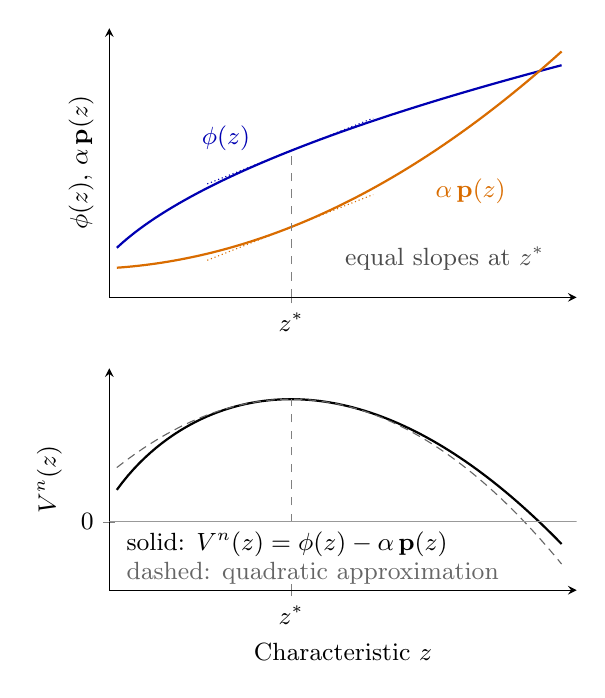
\begin{tikzpicture}
\begin{axis}[name=top,
  width=0.62\textwidth, height=5.0cm,
  xmin=0.2, xmax=3.3, ymin=0.8, ymax=4.6,
  axis lines=left, xtick={1.4057}, xticklabels={$z^*$}, ytick=\empty,
  ylabel={$\phi(z)$, $\alpha\,\mathbf{p}(z)$},
  tick label style={font=\small}, label style={font=\small}]
  \addplot[blue!70!black, thick, domain=0.25:3.2, samples=80] {2*sqrt(x) + 0.5};
  \addplot[orange!85!black, thick, domain=0.25:3.2, samples=80] {0.3*x^2 + 1.2};
  \addplot[blue!70!black, densely dotted, domain=0.85:1.95, samples=2] {2.8713 + 0.8433*(x - 1.4057)};
  \addplot[orange!85!black, densely dotted, domain=0.85:1.95, samples=2] {1.7928 + 0.8433*(x - 1.4057)};
  \draw[black!50, dashed] (axis cs:1.4057,0.8) -- (axis cs:1.4057,2.8713);
  \node[font=\small, blue!70!black, anchor=west] at (axis cs:0.75,3.05) {$\phi(z)$};
  \node[font=\small, orange!85!black, anchor=west] at (axis cs:2.3,2.3) {$\alpha\,\mathbf{p}(z)$};
  \node[font=\small, black!70, anchor=west, align=left] at (axis cs:1.7,1.35) {equal slopes at $z^*$};
\end{axis}
\begin{axis}[at={(top.south west)}, anchor=north west, yshift=-0.9cm,
  width=0.62\textwidth, height=4.4cm,
  xmin=0.2, xmax=3.3, ymin=-0.6, ymax=1.35,
  axis lines=left, xtick={1.4057}, xticklabels={$z^*$}, ytick={0}, yticklabels={$0$},
  xlabel={Characteristic $z$}, ylabel={$V^n(z)$},
  tick label style={font=\small}, label style={font=\small}]
  \addplot[black, thick, domain=0.25:3.2, samples=80] {2*sqrt(x) + 0.5 - 0.3*x^2 - 1.2};
  \addplot[black!60, densely dashed, domain=0.25:3.2, samples=80] {1.0784 - 0.45*(x - 1.4057)^2};
  \draw[black!50, dashed] (axis cs:1.4057,0) -- (axis cs:1.4057,1.0784);
  \draw[black!40] (axis cs:0.2,0) -- (axis cs:3.3,0);
  \node[font=\small, anchor=west] at (axis cs:0.25,-0.2) {solid: $V^n(z) = \phi(z) - \alpha\,\mathbf{p}(z)$};
  \node[font=\small, black!60, anchor=west] at (axis cs:0.25,-0.45) {dashed: quadratic approximation};
\end{axis}
\end{tikzpicture}
\caption{Net utility and its quadratic approximation. The top panel shows a concave utility of characteristics
$\phi(z)$ and a convex hedonic cost $\alpha\,\mathbf{p}(z)$, with equal slopes at the expected optimum $z^*$. The
bottom panel shows that net utility $V^n(z) = \phi(z) - \alpha\,\mathbf{p}(z)$ has an interior maximum at $z^*$. Its
dashed curve is the second-order expansion of \cref{prop:10-quadratic}. Illustrative functions $\phi(z) = 2\sqrt{z} + 0.5$ and
$\alpha\,\mathbf{p}(z) = 0.3z^2 + 1.2$. Redrawn after \citet{Trajtenberg1985}, Figure 1.}
\label{fig:10-hedonic-net-utility}
\end{figure}

\casehead{The separable specification} Trajtenberg simplifies further (p.~38). Suppose utility is additively
separable in characteristics, $\phi(z) = \sum_k f^k(z_k)$ with each $f^k$ quasi-concave, and the hedonic function
is linear in logs, $\mathbf{p}(z) = h_0 + \sum_k h_k\ln z_k$. Then net utility is separable too,
\begin{equation}\label{eq:10-traj-separable}
V^n(z) = \sum_k\left[f^k(z_k) - \alpha h_k\ln z_k\right] - \alpha h_0
\approx \sum_k\left(\beta_kz_k + \gamma_kz_k^2\right) + \text{const},
\end{equation}
because the Hessian of a separable function is diagonal and the cross terms of \eqref{eq:10-quadratic} vanish. The
saving of $\frac{K(K-1)}{2}$ parameters matters here. A multinomial logit (MNL) with characteristics that vary only
across products, and not across buyers, can include at most $|S| - 1$ such variables. Here $|S|$ is the number of
alternatives in the choice set $S$ (p.~38, n.~36). The separability of the hedonic function in $\ln z_k$ is what licenses the simplification. A double-log or
semi-log hedonic function would reintroduce cross terms (p.~39, n.~36).

\casehead{The estimating equation} Combining \eqref{eq:10-traj-netutility} and \eqref{eq:10-traj-separable}, the
model estimated for each year is
\begin{equation}\label{eq:10-traj-estimating}
s_j = \frac{e^{V_j}}{\sum_{k\in S_t}e^{V_k}},
\qquad
V_j = \sum_{k=1}^{K}\left(\beta_kz_{jk} + \gamma_kz_{jk}^2\right) + \vartheta\,\tilde p_j,
\qquad
\tilde p_j = p_j - \hat{\mathbf{p}}(z_j),
\end{equation}
with $K = 3$ characteristics. If the residual price measured only the price, $\vartheta$ would equal $-\alpha$.
\Cref{sec:10-ct-signal} explains why Trajtenberg allows otherwise. The procedure has two steps. The first estimates
the hedonic function and computes the residual prices. The second estimates the MNL by maximum likelihood with
$\tilde p_j$ as a regressor (p.~23). Trajtenberg abstracts from simultaneity. His working assumption is that each
choice set and its hedonic function are fixed before the year begins and do not change during it, which matches
the annual introduction cycle (p.~24). He also warns that the residual price may be correlated with omitted
attributes that affect choice, which would bias its coefficient (p.~24).

\subsection{Estimation and specification tests}\label{sec:10-ct-estimation}

\casehead{Step 1: hedonic regressions} Trajtenberg compares three forms (pp.~35--37). They are the double-log $\ln
p_j = h_0 + \sum_kh_k\ln z_{jk} + e_j$, the semi-log $\ln p_j = h_0 + \sum_kh_kz_{jk} + e_j$, and the linear-log
\begin{equation}\label{eq:10-traj-linearlog}
p_j = h_0 + \sum_k h_k\ln z_{jk} + e_j .
\end{equation}
As far as Trajtenberg knew, the linear-log form had not been used for hedonic prices before. When more of a characteristic is better, $h_k > 0$
and the form is concave, which is implausible. Here less is better, so $h_k < 0$, and $\frac{\partial^2}{\partial
z_k^2}h_k\ln z_k = -\frac{h_k}{z_k^2} > 0$ makes the function convex. The forms were estimated for 1976--81 on two
samples, all scanners with a head dummy and body scanners alone, which gives twelve cases. The \emph{Box-Cox
transformation} $\frac{p^\lambda - 1}{\lambda}$ gives the linear form at $\lambda = 1$ and the log form as
$\lambda\to 0$, so its likelihood puts the forms on a common scale. Box-Cox comparisons of fit ranked the linear-log first in half the cases, second in a third, and last in a sixth. The double-log ranked
first in a quarter, second in seven twelfths and third in a sixth (p.~37, n.~33). The linear-log has two further
advantages. Its residuals are in price units and enter the MNL directly, and it justifies the separable form
\eqref{eq:10-traj-separable}. \Cref{tab:10-ct-hedonic} reproduces the body-scanner regressions. The $R^2$ hovers
around 0.85 and most coefficients are significant, so the characteristics explain most of the variation in price.
Including price and characteristics together in the MNL would have produced the collinearity Trajtenberg feared.

\begin{table}[htbp]
\centering
\caption{Hedonic price regressions for body scanners, linear-log form}
\label{tab:10-ct-hedonic}
\small
\begin{tabular}{@{}lrrrrrr@{}}
\toprule
& 1976 & 1977 & 1978 & 1979 & 1980 & 1981 \\
\midrule
Intercept & 790.08 & 808.37 & 833.96 & 914.17 & 873.76 & 1,070.9 \\
          & (20.7) & (20.6) & (13.8) & (19.9) & (8.5) & (6.2) \\
$\ln$ SPEED & $-75.22$ & $-62.19$ & $-56.84$ & $-82.14$ & $-109.94$ & $-190.87$ \\
          & ($-11.0$) & ($-5.7$) & ($-3.2$) & ($-4.8$) & ($-3.5$) & ($-2.8$) \\
$\ln$ RESOL & $-12.58$ & $-161.79$ & $-150.02$ & $-198.65$ & $-382.30$ & $-337.77$ \\
          & ($-0.4$) & ($-2.7$) & ($-1.8$) & ($-3.4$) & ($-4.2$) & ($-2.2$) \\
$\ln$ RTIME & $-14.62$ & $-19.93$ & $-32.25$ & $-43.04$ & $-22.70$ & $-25.44$ \\
          & ($-2.5$) & ($-1.9$) & ($-2.0$) & ($-3.6$) & ($-0.8$) & ($-0.6$) \\
\addlinespace
$R^2$ & 0.981 & 0.878 & 0.656 & 0.847 & 0.811 & 0.783 \\
Degrees of freedom & 4 & 11 & 12 & 12 & 11 & 7 \\
\bottomrule
\end{tabular}

\smallskip
\begin{minipage}{0.9\linewidth}
\footnotesize Notes: Dependent variable is price in thousands of dollars. $t$-statistics in parentheses. For the
pooled sample of head and body scanners with a head dummy, the $R^2$ are 0.653, 0.895, 0.855, 0.937, 0.912 and 0.916
for 1976--81. Source: \citet{Trajtenberg1985}, Table 3, panels (b) and (a).
\end{minipage}
\end{table}

\casehead{Step 2: multinomial logit by year} The MNL is estimated separately for each year from 1975 to 1981, by
type of scanner, without buyer attributes except in 1975 (pp.~33--34). With about 300 purchases a year, computing
the surplus for every buyer and integrating over attributes would have multiplied the burden by an order of
magnitude. The estimates therefore describe a representative buyer, hospital or private clinic. Trajtenberg also
leaves out firm variables such as reputation or advertising, which improve the fit but have no clear welfare
interpretation (p.~34, n.~30). Choice sets changed within years. The software allowed buyers to face expanding
sets, so entries during the year were handled exactly, but exits were not (pp.~38--40). Fit is summarized by
$\rho^2 = 1 - \frac{L(\hat\beta)}{L(0)}$, with $L(0)$ the log likelihood when all alternatives are equally likely,
and by the correlation between predicted and actual shares.

Head scanners offered few models, so their MNL could be estimated only for 1976--79, in linear form with the
actual price, and without RTIME in 1979 (p.~45). Body scanners use the quadratic form \eqref{eq:10-traj-estimating}
with the residual price. \Cref{tab:10-ct-mnl} reproduces both tables. The coefficients on the characteristics
change substantially from year to year. Trajtenberg attributes this to the dual inducement mechanism of
\cref{sec:10-cs-hedonic}. Since the quadratic form makes individual coefficients hard to read, he measures relative
preferences by average derivatives of the choice probabilities (p.~45, n.~46). The price coefficients of head
scanners are negative and fairly stable, between $-0.71$ and $-0.89$. The residual-price coefficients of body
scanners are positive in every year except 1981.

\begin{table}[htbp]
\centering
\caption{Multinomial logit estimates for head and body scanners}
\label{tab:10-ct-mnl}
\small
\setlength{\tabcolsep}{5pt}
\begin{tabular}{@{}lrrrrrr@{}}
\toprule
\multicolumn{7}{@{}l}{\textit{Panel A. Head scanners, linear form}} \\
& 1976 & 1977 & 1978 & 1979 & & \\
\midrule
PRICE & $-0.748$ & $-0.709$ & $-0.893$ & $-0.818$ & & \\
      & ($-1.5$) & ($-1.9$) & ($-5.5$) & ($-2.4$) & & \\
SPEED & 0.018 & $-0.238$ & 0.303 & $-0.318$ & & \\
      & (0.2) & ($-1.4$) & (1.9) & ($-0.9$) & & \\
RESOL & $-4.706$ & $-5.565$ & $-7.756$ & $-10.307$ & & \\
      & ($-3.6$) & ($-2.9$) & ($-4.8$) & ($-4.7$) & & \\
RTIME & $-0.619$ & $-0.366$ & 1.119 & & & \\
      & ($-2.2$) & ($-1.2$) & (2.7) & & & \\
$\rho^2$ & 0.131 & 0.116 & 0.42 & 0.455 & & \\
Scanners, purchases & 6, 89 & 6, 56 & 8, 69 & 4, 80 & & \\
\midrule
\multicolumn{7}{@{}l}{\textit{Panel B. Body scanners, quadratic form with residual price}} \\
& 1976 & 1977 & 1978 & 1979 & 1980 & 1981 \\
\midrule
RPRICE & 11.252 & 0.993 & 1.020 & 0.485 & 0.695 & $-0.277$ \\
       & (6.4) & (4.8) & (4.8) & (1.8) & (2.4) & ($-2.5$) \\
SPEED & $-2.292$ & 2.138 & 4.624 & $-8.669$ & 11.347 & $-7.504$ \\
      & ($-7.3$) & (2.8) & (1.0) & ($-1.5$) & (2.0) & ($-0.5$) \\
SPEED$^2$ & 0.236 & $-1.264$ & $-8.283$ & 31.292 & $-34.838$ & 74.161 \\
      & (4.0) & ($-3.4$) & ($-0.6$) & (1.9) & ($-1.6$) & (1.4) \\
RESOL & 69.107 & 9.113 & $-34.126$ & $-15.283$ & $-18.129$ & 32.877 \\
      & (7.3) & (2.4) & ($-6.3$) & ($-5.0$) & ($-3.6$) & (3.9) \\
RESOL$^2$ & $-23.360$ & $-2.533$ & 15.096 & 6.291 & 7.738 & $-24.028$ \\
      & ($-7.6$) & ($-1.5$) & (5.8) & (3.8) & (2.7) & ($-4.2$) \\
RTIME & $-3.931$ & 5.082 & 2.385 & 3.288 & 3.161 & $-2.591$ \\
      & ($-5.3$) & (7.0) & (2.0) & (3.3) & (2.8) & ($-2.8$) \\
RTIME$^2$ & 1.054 & $-2.370$ & $-1.511$ & $-1.401$ & $-2.093$ & 5.560 \\
      & (4.5) & ($-6.7$) & ($-2.0$) & ($-2.1$) & ($-2.2$) & (3.9) \\
$\rho^2$ & 0.29 & 0.12 & 0.16 & 0.16 & 0.20 & 0.14 \\
Scanners, purchases & 8, 285 & 15, 324 & 16, 164 & 16, 177 & 15, 193 & 11, 153 \\
\bottomrule
\end{tabular}

\smallskip
\begin{minipage}{0.94\linewidth}
\footnotesize Notes: Asymptotic $t$-statistics in parentheses. Prices are in hundreds of thousands of dollars.
RPRICE is the residual price from the year's hedonic regression. The correlations between predicted and actual
shares are 0.999, 0.910, 0.993 and 0.998 for head scanners and 0.999, 0.877, 0.900, 0.870, 0.722 and 0.547 for body
scanners. The 1981 data cover the first half of the year. Source: \citet{Trajtenberg1985}, Tables 4 and 5.
\end{minipage}
\end{table}

\casehead{Testing independence of irrelevant alternatives} Should head and body scanners form one choice set? Under
IIA the cross-price elasticities of all products with respect to the price of product $k$ are equal. A body scanner
and a head scanner would then be equally good substitutes for any third scanner (p.~41). Trajtenberg applies the
test of \citet{HausmanMcFadden1984}. Let $\hat\beta_f$ be the MNL estimate on the full set of head and body scanners.
Let $\hat\beta_r$ be the estimate on the restricted set of body scanners, using the buyers who chose from it. Under the
null hypothesis that IIA holds on the full set, both estimators are consistent and $\hat\beta_f$ is efficient. The
statistic is
\begin{equation}\label{eq:10-hm-test}
S = \left(\hat\beta_r - \hat\beta_f\right)^\top\left(\widehat V_r - \widehat V_f\right)^{-1}\left(\hat\beta_r -
\hat\beta_f\right) \;\xrightarrow{d}\; \chi^2_m,
\end{equation}
with $m$ the rank of $\widehat V_r - \widehat V_f$ (p.~42). The variance of the difference is the difference of the
variances by the argument of \citet{Hausman1978}. An efficient estimator must be uncorrelated with its difference
from any other consistent estimator. Otherwise a linear combination of the two would be consistent with smaller
variance. \Cref{app:econometrics} gives the general Hausman test.

Trajtenberg computes the test for 1977 and 1981. He chose years far apart, with similar ratios of head to body
models, so that the results would not depend on the relative number of alternatives dropped (p.~42, n.~40). The
statistics are $S(1977) = 21.83$ and $S(1981) = 27.77$, against a 1 percent cutoff of 18.5. IIA is rejected for the
full set. This cutoff is the 0.99 quantile of a $\chi^2$ with seven degrees of freedom, consistent with the seven coefficients
of the body-scanner specification. He notes that the test is an omnibus test, with power only against large departures
from the MNL. Its advantage is that it needs no model beyond the MNL.

\casehead{The nested logit} Trajtenberg next estimates a nested logit with a head branch $H$ and a body branch $B$
(pp.~43--47), in the parameterization of \eqref{eq:10-nl-semi} with no nest constants:
\begin{equation}\label{eq:10-traj-nested}
s_{j} = s_{j|g}\,s_g,
\qquad
s_{j|g} = \frac{e^{V_j}}{\sum_{k\in g}e^{V_k}},
\qquad
s_g = \frac{e^{\lambda W_g}}{e^{\lambda W_H} + e^{\lambda W_B}},
\qquad
W_g = \ln\sum_{k\in g}e^{V_k} .
\end{equation}
At $\lambda = 1$ the model collapses to the MNL on the full set. At $\lambda = 0$ the cross elasticities between
branches are zero, the branch shares no longer depend on the products, and each branch is a separate market. With
branch constants chosen to reproduce the observed branch shares, the surplus function is then
$\mathcal{W} = \sum_g s_gW_g$ in utility units, which is \cref{cor:10-separate-markets}
(equation 23 of the paper, p.~44). Estimation is sequential. The first stage is the branch MNLs of
\cref{tab:10-ct-mnl}. The inclusive values are computed from them, and the second stage estimates $\lambda$ in the
branch-choice model. The second-stage standard errors are not corrected for the first stage, so Trajtenberg does not
test $\lambda = 0$ formally (p.~47, n.~47).

\Cref{tab:10-ct-nested} reports the second stage. Except in 1978, $\hat\lambda$ is between 0.02 and 0.08.
Trajtenberg concludes that the cross elasticities between head and body scanners are nil, so the two types form
separate markets. He reads the negative estimate for 1978 as a local failure of the conditions for a generalized
extreme value model, since $\lambda$ must lie in the unit interval. A negative $\lambda$ would even suggest
complementarity. The conclusion agrees with the divergent technological paths of the two types. Trajtenberg stresses a
broader lesson. Estimating $\lambda$ offers a way to draw market boundaries in empirical studies (p.~47).

\begin{table}[htbp]
\centering
\caption{Nested logit, second stage, and a reinterpretation}
\label{tab:10-ct-nested}
\small
\begin{tabular}{@{}lrrrrrrr@{}}
\toprule
& \multicolumn{2}{c}{Inclusive values} & \multicolumn{3}{c}{Second stage} & \multicolumn{2}{c}{Reinterpretation} \\
\cmidrule(lr){2-3}\cmidrule(lr){4-6}\cmidrule(lr){7-8}
Year & $W_B$ & $W_H$ & $\hat\lambda$ & (s.e.) & $\rho^2$ & Body share & Implied $\lambda$ \\
\midrule
1976 & 47.704 & $-9.102$ & 0.0205 & (0.00214) & 0.21 & 0.762 & 0.0205 \\
1977 & 11.989 & $-10.410$ & 0.0784 & (0.00646) & 0.40 & 0.849 & 0.0771 \\
1978 & $-14.428$ & $-10.340$ & $-0.2120$ & (0.03510) & 0.12 & 0.724 & $-0.2359$ \\
1979 & $-4.728$ & $-15.806$ & 0.0706 & (0.01211) & 0.10 & 0.702 & 0.0773 \\
\bottomrule
\end{tabular}

\smallskip
\begin{minipage}{0.94\linewidth}
\footnotesize Notes: $W_g = \ln\sum_{k\in g}e^{V_k}$ from the first-stage MNLs. The body share is the share of body
scanners in unit sales (\cref{tab:10-ct-data}, Panel B). The implied $\lambda$ is $\frac{1}{W_B - W_H}\ln\frac{s_B}{1
- s_B}$, the value at which the branch model reproduces the observed body share. Hausman-McFadden statistics for the
full versus body-only choice set are 21.83 (1977) and 27.77 (1981), against a 1 percent cutoff of 18.5. Source:
\citet{Trajtenberg1985}, Table 6 and pp.~41--42. The implied $\lambda$ is our computation.
\end{minipage}
\end{table}

The last two columns of \cref{tab:10-ct-nested} suggest a more cautious reading, which is ours and not the paper's.
In the second stage each buyer chooses a branch, and the only regressor is $W_B - W_H$. If all buyers in a year face
the same choice set, this regressor is the same for every buyer. The score of the binary logit likelihood is then
\begin{equation*}
\sum_i\left[\indic\{i\text{ buys body}\} - \Lambda\left(\lambda(W_B - W_H)\right)\right](W_B - W_H) = 0,
\end{equation*}
with $\Lambda$ the logistic CDF. The estimate sets the predicted body share equal to the observed one, so
\begin{equation}\label{eq:10-traj-lambda-implied}
\hat\lambda = \frac{1}{W_B - W_H}\ln\frac{s_B}{1 - s_B}.
\end{equation}
Within-year entry makes choice sets differ slightly across buyers, so the formula holds only approximately. It
reproduces the 1976 estimate exactly and the others closely. The magnitude of $\hat\lambda$ is therefore the log
odds of the body share divided by the gap between the inclusive values. That gap has an arbitrary location. Each
branch MNL is invariant to adding a constant to all its $V$'s, and the two branches use different functional forms
with no intercepts. A branch constant would fit the shares exactly for any $\lambda$. The 1978 sign, for instance,
arises because $W_B < W_H$ that year while body scanners outsold head scanners. On this reading the second stage
carries little information about substitution between the branches. Trajtenberg's conclusion that the two types
were separate markets may still be right, given the evidence from technology, prices and use. It does not, however,
rest on the estimated $\lambda$.

\casehead{The first year with a choice} In 1973 and 1974 only the EMI head scanner was sold, so there was nothing to
estimate (p.~33, n.~28). In 1975 the first two body scanners and a second head scanner entered. At that stage the
two types were still similar in characteristics and price, and the effective choice set had four alternatives
(pp.~47--48). With room for only three variables that vary across products alone, Trajtenberg estimated a hybrid
specification on hospitals only. He interacted resolution with a hospital attribute, which makes it vary across buyers
and bypasses the limit. In his Table 7 the residual-price coefficient is 10.183 ($t = 4.3$) and the interaction
of a head dummy with price is $-2.875$ ($t = -6.0$). The coefficients are $-0.165$ for SPEED ($t = -0.8$) and
$-6.338$ for RESOL times RAD ($t = -4.8$), with $\rho^2 = 0.24$ from 181 purchases. RAD is the average of three dummy variables
for the availability of x-ray, cobalt and radium therapy at the hospital. It lets resolution matter more to hospitals
with a wider range of radiation therapy, and the RESOL coefficient at the mean of RAD is $-4.183$.

\subsection{Positive price coefficients and signaling}\label{sec:10-ct-signal}

A positive residual-price coefficient cannot be read as a negative marginal utility of income, and the surplus
function needs $\alpha$ to convert utility into money. Nor is it clear whether $\vartheta\tilde p_j$ belongs in
the utility used for welfare (pp.~48--49). Trajtenberg addresses both questions with a model of price, quality and
quantity interdependence in the tradition of Spence. Demand $q$ depends on price and on perceived quality $\psi$,
which may in turn depend on price and quantity,
\begin{equation}\label{eq:10-spence}
q = q(p,\psi),
\qquad
\psi = \Psi(p,q) .
\end{equation}
The observed demand curve is $q = q(p,\Psi(p,q))$. Totally differentiating the two equations gives
\begin{align*}
dq &= q_p\,dp + q_\psi\,d\psi, \\
d\psi &= \Psi_p\,dp + \Psi_q\,dq .
\end{align*}
Substituting the second into the first,
\begin{equation*}
dq\left(1 - q_\psi\Psi_q\right) = \left(q_p + q_\psi\Psi_p\right)dp,
\end{equation*}
so
\begin{equation}\label{eq:10-spence-slope}
\frac{dq}{dp} = \frac{q_p + q_\psi\Psi_p}{1 - q_\psi\Psi_q}
\end{equation}
(equation 28, p.~50). With $\Psi_q = 0$ and $\Psi_p > 0$, perceived quality rises with price, and the observed
demand curve slopes up whenever $q_\psi\Psi_p > -q_p$. In econometric terms this is the bias from omitting a quality
variable correlated with price (p.~51).

Trajtenberg argues that the observed characteristics are only partly informative about a scanner's performance,
for buyers as well as for the econometrician. Prices can then signal quality. He postulates that expected quality
depends on the part of price not explained by the observed characteristics, $\psi^e = \Psi(p - \mathbf{p}(z)) =
\Psi(\tilde p)$ (equation 30, p.~52). He then asks whether a signaling equilibrium, in which expected and realized
quality agree on average, is plausible. A firm could price above its true quality and exit once the bluff is
called. Trajtenberg argues that this ``quick kill'' was unlikely in CT. Reputation mattered in medical equipment,
most firms operated in many related markets, and research and marketing costs were persistently high (pp.~52--53).

In a signaling equilibrium the expected quality is a real quality dimension and belongs in utility (p.~53):
\begin{equation*}
V_j = V^1(z_j) + V^2(\psi^e_j) - \alpha p_j .
\end{equation*}
Take $V^2(\psi^e) = b_\psi\psi^e$ and $\psi^e_j = a_\psi\tilde p_j$, and write $\beta_0 = a_\psi b_\psi$ for the
marginal utility of a dollar of residual price through the signal. Substituting $p_j = \mathbf{p}(z_j) + \tilde p_j$,
\begin{equation}\label{eq:10-signal-V}
V_j = \left[V^1(z_j) - \alpha\,\mathbf{p}(z_j)\right] + (\beta_0 - \alpha)\tilde p_j,
\qquad
\vartheta = \beta_0 - \alpha
\end{equation}
(equations 32 and 33). The estimated coefficient is positive when the signaling effect exceeds the price effect,
$\beta_0 > \alpha$. Two implications follow (p.~54). The estimated $\vartheta\tilde p_j$ should stay in $V_j$ when
computing $\mathcal{W}(S_t)$, because the signaled quality is real. But the conversion to money requires $\alpha$
itself. Dividing by $\vartheta$ in the surplus function would be meaningless.

To identify $\alpha$ Trajtenberg uses the contrast between the two types (pp.~54--55). Signaling should matter more
for products that are complex, new to users and changing fast, and it should fade as a product matures. Head scanners
were introduced first, kept the same application, and after early improvements became simpler and cheaper. Body
scanners grew steadily more sophisticated, with large jumps in the first years. Trajtenberg therefore treats the
head-scanner price coefficients for 1976--79 as unbiased estimates of $\alpha$. The head scanner had been on the
market for three years by 1976, which he takes as long enough for signaling to vanish (p.~55, n.~53). He uses the
1976 coefficient for earlier years and the 1979 coefficient for later ones (p.~56). The difference between the body
and head coefficients then measures the signaling effect.

The signaling interpretation deserves scrutiny. The more natural reading of a positive price coefficient is
omitted quality correlated with price, the endogeneity problem later handled with instruments by \citet{Berry1994}
and \citet{BerryLevinsohnPakes1995}. \Citet[p.~708]{Petrin2002} cites Trajtenberg as an example of a price
coefficient biased toward zero by omitted characteristics. In these data the two readings are observationally
equivalent. Both imply that the residual price proxies real quality, so both support keeping $\vartheta\tilde p_j$
in $V_j$. They differ on whether a clean $\alpha$ is available. Importing $\alpha$ from head scanners assumes that
buyers of the two types have the same marginal utility of income, an assumption the data cannot test. The head coefficients are also imprecise, with $t$-statistics of $-1.5$ and $-1.9$ in 1976 and
1977. Finally, the 1981 body coefficient is $-0.277$. If signaling had vanished by then, this coefficient should be
near the head value of about $-0.8$. Its smaller magnitude suggests that a positive bias remained.

\subsection{Welfare computations}\label{sec:10-ct-welfare}

Trajtenberg computes both measures of \eqref{eq:10-exante-expost} (pp.~58--60). The residual prices must come from
the hedonic function of the reference year, since $\mathbf{p}(z)$ is added back to the quadratic approximation to
recover utility. For the ex ante measure the year-$t$ hedonic function generates the residuals of both years, and
for the ex post measure the year-$(t+1)$ function does. Because the IIA test rejected a common tree from 1976 on,
the gains are computed separately for head and body scanners for 1976--82. For 1973--76 they are computed for the
joint set with the 1975 parameters. The 1973 and 1974 sets contain one head scanner each.

The computation for body scanners has three steps (p.~59). The first computes the change in the log-sum,
\begin{equation}\label{eq:10-traj-dWtilde}
\Delta\widetilde{\mathcal{W}}_{t,t+1} = \ln\sum_{j\in S_{t+1}}e^{V_j} - \ln\sum_{j\in S_t}e^{V_j}.
\end{equation}
The second divides by the absolute value of $\alpha$ and multiplies by 100, because prices were measured in
hundreds of thousands of dollars. The result is the gain in thousands of dollars per buyer. The third deflates by the
producer price index for capital equipment (1982 = 1.00). \Cref{tab:10-ct-body} reproduces Table 8. The arithmetic of
the table reveals a detail the text does not state. The ex ante column divides by the year-$t$ coefficient, the
value printed in column (2), while the ex post column divides by the year-$(t+1)$ coefficient. For 1977--78, for
example, $\frac{-0.419}{0.893}\times100 = -46.9$, which uses the 1978 coefficient.

\begin{table}[htbp]
\centering
\caption{Welfare gains from innovation in body scanners, 1976--1982}
\label{tab:10-ct-body}
\small
\setlength{\tabcolsep}{5pt}
\begin{tabular}{@{}lrrrrrrrr@{}}
\toprule
& \multicolumn{2}{c}{(1) $\Delta\widetilde{\mathcal{W}}_B$} & (2) & \multicolumn{2}{c}{(3) Gain (\$K)} & (4) &
  \multicolumn{2}{c}{(5) Real gain (\$K)} \\
\cmidrule(lr){2-3}\cmidrule(lr){5-6}\cmidrule(lr){8-9}
Period & Ex ante & Ex post & $|\alpha|$ & Ex ante & Ex post & PPI & Ex ante & Ex post \\
\midrule
1975--76 & 14.715$^a$ & 2.930 & 0.748 & 1,967.2 & 391.7 & 0.620 & 3,173.0 & 631.8 \\
1976--77 & 5.416 & 0.764 & 0.748 & 724.1 & 107.8 & 0.660 & 1,097.1 & 163.3 \\
1977--78 & 0.110 & $-0.419$ & 0.709 & 15.5 & $-46.9$ & 0.712 & 21.8 & $-65.9$ \\
1978--79 & 1.413 & 0.349 & 0.893 & 158.2 & 42.7 & 0.774 & 204.4 & 55.1 \\
1979--80 & 0.681 & 0.377 & 0.818 & 83.3 & 46.1 & 0.858 & 97.0 & 53.7 \\
1980--81 & 1.551 & $-0.073$ & 0.818 & 189.6 & $-8.9$ & 0.945 & 200.6 & $-9.4$ \\
1981--82 & 1.709 & -- & 0.818 & 208.9 & -- & 1.00 & 208.9 & -- \\
\bottomrule
\end{tabular}

\smallskip
\begin{minipage}{0.94\linewidth}
\footnotesize Notes: Column (1) is the change in the log-sum \eqref{eq:10-traj-dWtilde}. Column (2) is the head-scanner
price coefficient used for the ex ante measure. The ex post measure uses the coefficient of the following year. Column (3) is $\frac{(1)}{(2)}\times100$, and column (5) is
$\frac{(3)}{(4)}$, where (4) is the producer price index for capital equipment with 1982 = 1.00. $^a$Imputed value. In real terms it equals the joint 1975--76 ex ante gain of
\cref{tab:10-ct-gains} times the body scanners' share of the 1975--76 ex post gains,
$\frac{0.6318}{0.3191 + 0.6318}\times4.7758 = 3.173$ (our reading). The
last digit of the ex post entry for 1975--76 in column (5) is faint in the source and equals $\frac{391.7}{0.620}$.
Source: \citet{Trajtenberg1985}, Table 8.
\end{minipage}
\end{table}

Table 9 of the paper, reproduced as \cref{tab:10-ct-gains}, brings the two types together. The overall gain in each
period is the share-weighted average
\begin{equation}\label{eq:10-traj-overall}
\Delta\mathcal{W} = s_H\,\Delta\mathcal{W}_H + s_B\,\Delta\mathcal{W}_B,
\end{equation}
where $s_g$ is the fraction of buyers who bought type $g$. This is \eqref{eq:10-separate-markets} applied to
separate markets, with branch constants that reproduce the observed shares. The 1975--76 ex ante gain, computed for the joint set with the 1975 parameters, is entered for both
types. Ex ante and ex post pairs overlap for four periods, 1975--76 to 1978--79. In those periods the ex ante gain
exceeds the ex post gain by a fairly constant factor, as the dual inducement argument predicts. The mean ratio is
7.24 with standard deviation 1.34 (p.~60). Trajtenberg uses this ratio to impute the ex ante gains of 1973--74 and
1974--75 and the ex post gains of 1979--82. The incremental gains are the $\Delta\mathcal{W}_t$, and their running
sums are the cumulative gains.

\begin{table}[htbp]
\centering
\caption{Welfare gains by scanner type, incremental and cumulative overall gains (\$M per buyer)}
\label{tab:10-ct-gains}
\footnotesize
\setlength{\tabcolsep}{3.6pt}
\begin{tabular}{@{}lrrrrrrrrrr@{}}
\toprule
& \multicolumn{3}{c}{Head scanners} & \multicolumn{3}{c}{Body scanners} & \multicolumn{2}{c}{Incremental} &
  \multicolumn{2}{c}{Cumulative} \\
\cmidrule(lr){2-4}\cmidrule(lr){5-7}\cmidrule(lr){8-9}\cmidrule(lr){10-11}
Period & $\Delta\mathcal{W}^a_H$ & $\Delta\mathcal{W}^p_H$ & $s_H$ & $\Delta\mathcal{W}^a_B$ &
  $\Delta\mathcal{W}^p_B$ & $s_B$ & Ex ante & Ex post & Ex ante & Ex post \\
\midrule
1973--74 & -- & 1.2038 & 1.00 & -- & 1.2038 & 0 & 8.7126$^*$ & 1.2038 & 8.7126 & 1.2038 \\
1974--75 & -- & 0.2085 & 0.552 & -- & 0.2085 & 0.448 & 1.5090$^*$ & 0.2085 & 10.2216 & 1.4123 \\
1975--76 & 4.7758 & 0.3191 & 0.238 & 4.7758 & 0.6318 & 0.762 & 4.7758 & 0.5574 & 14.9974 & 1.9697 \\
1976--77 & 0.0559 & 0.0169 & 0.151 & 1.0971 & 0.1633 & 0.849 & 0.9399 & 0.1412 & 15.9373 & 2.1109 \\
1977--78 & 0.3609 & 0.2248 & 0.276 & 0.0218 & $-0.0659$ & 0.724 & 0.1154 & 0.0143 & 16.0527 & 2.1252 \\
1978--79 & $-0.0127$ & $-0.0469$ & 0.298 & 0.2044 & 0.0551 & 0.702 & 0.1397 & 0.0247 & 16.1924 & 2.1499 \\
1979--80 & $-0.0187$ & -- & 0.196 & 0.0970 & 0.0537 & 0.804 & 0.0743 & 0.0103$^*$ & 16.2667 & 2.1602 \\
1980--81 & 0.0072 & -- & 0.084 & 0.2006 & $-0.0094$ & 0.916 & 0.1844 & 0.0255$^*$ & 16.4511 & 2.1857 \\
1981--82 & $-0.0028$ & -- & 0.065 & 0.2089 & -- & 0.935 & 0.1951 & 0.0270$^*$ & 16.6462 & 2.2127 \\
\bottomrule
\end{tabular}

\smallskip
\begin{minipage}{0.96\linewidth}
\footnotesize Notes: Millions of 1982 dollars per representative buyer. $s_g$ is the share of buyers choosing type
$g$. $^*$Computed with the mean ratio of ex ante to ex post gains for 1976--79. For 1973--74 and 1974--75 the paper
enters the joint ex post gain in both type columns. Every overall entry satisfies \eqref{eq:10-traj-overall}
to four decimals, and the cumulative columns are running sums. Source: \citet{Trajtenberg1985}, Table 9.
\end{minipage}
\end{table}

\casehead{Interpretation} The cumulative ex ante gain to 1982 is \$16.6 million per buyer, and the ex post gain
\$2.2 million. Most of it accrues before 1977. The largest single increment, \$8.71 million ex ante in 1973--74, comes
from the second EMI model, discussed in \cref{sec:10-ct-diffusion}. It is imputed from the ex post gain with the mean
ratio. These per-buyer gains are large. In 1975--76 the
ex ante gain of \$4.78 million is several times the price of a body scanner in \cref{tab:10-ct-data}, even allowing
for the deflation to 1982 dollars. Large gains are possible for a revolutionary technology, since buyers can value an
early improvement far above its price. But two features of the estimates suggest that the functional form also plays
a role. The ex ante measure exceeds the ex post measure by a factor of seven. And the logit adds an entropy term for
every new model (\cref{prop:10-entropy}), while the quadratic utility extrapolates the value of large changes in
characteristics.

\subsection{Who is the consumer?}\label{sec:10-ct-consumer}

The buyers of CT scanners are hospitals and clinics, which buy them as capital inputs and sell diagnostic services to
patients (pp.~60--63). This does not by itself invalidate the welfare measure. Under perfect competition, the surplus
from the derived demand for an input equals the surplus from the final demand for the output. The firm is then a
redundant intermediary (p.~61, n.~56). Regulation affects the surplus that is realized, but the measure still captures
it.

Trajtenberg locates the difficulty in the behavior of hospitals. He compares two ideal types and the patient. Let
$q(z)$ be the price of a procedure performed with a scanner of quality $z$. The operating cost per procedure is
$C[z,\mathbf{p}(z)]$, which rises with quality and with the scanner's price. A profit-maximizing, price-taking hospital solves
\begin{equation*}
\max_z\; q(z) - C[z,\mathbf{p}(z)]
\qquad\Longrightarrow\qquad
q_z = C_z .
\end{equation*}
A hospital that maximizes a utility $v^h(z)$ of the quality of its diagnostic services instead sets $v^h_z = C_z$. A
patient with utility $v^c(z) + y^c - q(z)$ chooses $v^c_z = q_z$. Under perfect competition
\begin{equation}\label{eq:10-traj-agency}
v^c_z = q_z = C_z = v^h_z ,
\end{equation}
and the hospitals' demand for scanners, which is what the MNL estimates, reflects the patients' valuation. Trajtenberg
doubts that $v^h_z = v^c_z$. Physicians may value diagnostic technology above patients do, because of rivalry between
hospitals, long-range scientific goals, status and prestige. If so, the measured gains overstate the social gains
(p.~62). A deeper problem is that $v^c_z$ is hardly defined. Patients cannot evaluate the medical value of diagnostic
procedures, so the size of the principal-agent problem cannot be gauged (p.~63). Trajtenberg proceeds on the
assumption that extraneous motives are not the main driver of hospitals' choices. Insurance adds a further wedge
that the paper does not model. Insured patients do not face the full price of a procedure, so neither their demand nor
the hospital's derived demand measures willingness to pay at the margin.

\subsection{Diffusion, total gains and social returns}\label{sec:10-ct-diffusion}

The $\Delta\mathcal{W}_t$ are gains per representative buyer. Total gains require the number of buyers who benefit
from each year's innovations, and this depends on the dynamics of adoption (pp.~63--67). Trajtenberg contrasts two
polar views of diffusion. In the first, diffusion traces the distribution of reservation prices among potential
adopters. Each innovation lowers the quality-adjusted price, triggers adoption by the buyers just at the margin, and
benefits only those who buy in the year it appears. Total gains are then
\begin{equation}\label{eq:10-traj-TW-reservation}
TW_t = \Delta\mathcal{W}_t\,n_t ,
\end{equation}
where $n_t$ is the number of buyers in year $t$. In the second view diffusion is driven entirely by demonstration
effects, such as learning, emulation and rivalry. Today's innovations then benefit all future adopters too. With $N$
potential adopters, adoption-time density $f$, CDF $F$ and discount rate $r$,
\begin{equation}\label{eq:10-traj-TW-demo}
TW_t = \Delta\mathcal{W}_t\,N\int_t^{\infty}f(\tau)e^{-r(\tau - t)}\,d\tau .
\end{equation}
Ignoring discounting, $TW_t = \Delta\mathcal{W}_tN[1 - F(t)] = \Delta\mathcal{W}_t(n_t + n^f_t)$, with
$n^f_t = N[1 - F(t+1)]$ the number of future adopters. The demonstration view gives larger totals.

\casehead{The diffusion equation} To find out which view fits, Trajtenberg estimates a logistic diffusion curve whose
ceiling rises with the cumulative gains from innovation, $CW_t = \sum_{\tau\le t}\Delta\mathcal{W}_\tau$ (pp.~67--68):
\begin{equation}\label{eq:10-traj-diffusion}
F(t) = \frac{K_0 + k\,CW_t}{1 + \exp(a_0 - a_1t)} .
\end{equation}
Time captures demonstration effects, and the cumulative gains act as a quality-adjusted price index that shifts the
distribution of reservation prices. A linear ceiling corresponds to uniformly distributed reservation prices.
Trajtenberg also tried a concave ceiling, corresponding to exponentially distributed ones, with very similar results.
The equation cannot be linearized by taking log odds, so it is estimated by nonlinear least squares. Time is measured in
months from November 1972 to July 1981, and $F(t)$ is the fraction of the $N = 3{,}457$ potential adopters that have
bought a first scanner. The population consists of the 3,078 community hospitals with more than 100 beds and the 379
private clinics that had bought a scanner by July 1981 (p.~68, n.~65). The series $CW_t$ is the ex ante cumulative
gain of \cref{tab:10-ct-gains}.

Table 10 of the paper reports two specifications, with asymptotic standard errors in parentheses. The traditional
logistic with a free ceiling gives $K_0 = 0.459$ (0.004), $a_0 = 4.053$ (0.076), $a_1 = 0.071$ (0.002) and a residual
sum of squares of 0.013. With the innovation term, $K_0 = 0.074$ (0.003), $k = 0.025$ (0.002), $a_0 = 3.443$ (0.07)
and $a_1 = 0.06$ (0.001), and the residual sum of squares falls to 0.006. Both time and innovation matter, and the
traditional model that ignores innovation fits much worse (p.~68). The estimate $k = 0.025$ means that each million
dollars of improvement per buyer raises the eventual adoption rate by 2.5 percentage points. Had technical change
stopped after the first scanner, only 7.4 percent of potential adopters would have adopted. With $CW_{82} = 16.65$,
the ceiling reached $0.074 + 0.025\times16.65 = 0.49$ by 1982 (p.~69, n.~66). Trajtenberg also allowed the incremental
gains $\Delta\mathcal{W}_t$ to shift the speed of diffusion, and found that effect significant but very small (p.~68,
n.~64).

\casehead{The value of the first scanner} The diffusion equation yields an indirect estimate of the gain from the
first scanner, the radical innovation that the surplus function cannot value. If the behavior behind the equation is
stable, the first scanner must have been worth enough to generate the initial ceiling $K_0$. Its gain therefore
satisfies $k\,\Delta\mathcal{W}_{73} = K_0$, so
\begin{equation*}
\Delta\mathcal{W}_{73} = \frac{K_0}{k} = \frac{0.074}{0.025} = 2.99
\end{equation*}
million dollars per buyer (p.~69). With the rounded estimates the ratio is 2.96, so the paper's 2.99 presumably uses
more digits. Trajtenberg cautions that this figure is computed in a very different and probably less precise way than
the others.

\casehead{Total gains} Trajtenberg combines the two views (p.~70). Current buyers receive the incremental gain, and so do
the future adopters attracted by the higher ceiling, discounted at 5 percent a year (0.0041 a month):
\begin{equation}\label{eq:10-traj-TW}
TW_t = \Delta\mathcal{W}_t\left[n_t + N\left(K_0 + k\,CW_t\right)\int_{t+1}^{\infty}f(\tau)e^{-r(\tau - t - 1)}\,d\tau\right].
\end{equation}
The integral has no closed form and is computed numerically. Repeat purchases, which include second scanners and
replacements, are credited only with the incremental gain of their year. This is a lower bound, since the upper bound
would credit all gains since the buyer's previous purchase (p.~70, n.~67). Upgrades of installed scanners are ignored,
although nearly a quarter of the scanners installed by mid-1981 had been upgraded. The only source of upward bias is
the implicit assumption that adopters are just at the margin when they adopt, so that they receive the incremental gain
in full. Buyers who delay adoption in anticipation of further improvements would offset this bias (pp.~70--71).
\Cref{tab:10-ct-total} reproduces the computation. Total gains are \$6.9 billion in 1974 and \$6.0 billion in 1976, and
they fall below \$100 million a year from 1978 on.

\begin{table}[htbp]
\centering
\caption{Computation of total ex ante gains (\$M)}
\label{tab:10-ct-total}
\small
\begin{tabular}{@{}lrrrrrrrrr@{}}
\toprule
& (1) & (2) & (3) & (4) & (5) & (6) & (7) & (8) & (9) \\
Year & $\Delta\mathcal{W}_t$ & $K(CW_t)$ & $1 - F(t)$ & Discounted & $n^f_t$ & $\tilde n^f_t$ & $n_t$ &
  $n_t + \tilde n^f_t$ & $TW_t$ \\
\midrule
1973 & 2.9900 & 0.0740 & 0.9383 & 0.7720 & 240 & 197 & 16 & 213 & 638.3 \\
1974 & 8.7126 & 0.2898 & 0.8776 & 0.7506 & 879 & 752 & 43 & 795 & 6,926.3 \\
1975 & 1.5090 & 0.3271 & 0.7769 & 0.6853 & 879 & 775 & 221 & 996 & 1,502.9 \\
1976 & 4.7758 & 0.4453 & 0.6285 & 0.5676 & 967 & 874 & 374 & 1,248 & 5,959.1 \\
1977 & 0.9399 & 0.4686 & 0.4512 & 0.4141 & 731 & 671 & 390 & 1,061 & 997.1 \\
1978 & 0.1154 & 0.4714 & 0.2854 & 0.2646 & 465 & 431 & 250 & 681 & 78.6 \\
1979 & 0.1397 & 0.4749 & 0.1625 & 0.1515 & 267 & 249 & 275 & 524 & 73.2 \\
1980 & 0.0743 & 0.4767 & 0.0862 & 0.0806 & 142 & 133 & 271 & 404 & 30.0 \\
1981 & 0.1844 & 0.4813 & 0.0245 & 0.0230 & 41 & 38 & 392 & 430 & 79.3 \\
1982 & 0.1951 & 0.4861 & 0.0121 & 0.0113 & 20 & 19 & 428 & 447 & 87.2 \\
\bottomrule
\end{tabular}

\smallskip
\begin{minipage}{0.94\linewidth}
\footnotesize Notes: (1) Incremental ex ante gain per buyer, with the 1973 entry equal to $\frac{K_0}{k}$. (2)
$K(CW_t) = 0.074 + 0.025\,CW_t$. (3) Share of the logistic adoption distribution after year $t$, and (4) the same
share discounted to year $t+1$ at 5 percent a year. (5) $n^f_t = (2)\times(3)\times N$ and (6) $\tilde n^f_t =
(2)\times(4)\times N$, with $N = 3{,}457$. (7) Scanners sold in year $t$. (9) $TW_t = (1)\times(8)$. Source:
\citet{Trajtenberg1985}, Table 11 and its notes.
\end{minipage}
\end{table}

\casehead{Research and development and the social rate of return} Trajtenberg collected research and development
spending on CT for almost all firms active in the field (pp.~71--72). \Cref{tab:10-ct-rd} reproduces the annual totals.
He does not show the breakdown by firm, which was confidential. Since the benefits are measured for U.S. buyers while
the innovations came from U.S. and foreign firms, he computes returns both to U.S. research and to total research. He
reads them as upper and lower bounds on the true rate.

\begin{table}[htbp]
\centering
\caption{Research and development spending on CT scanners (constant 1982 \$M)}
\label{tab:10-ct-rd}
\small
\begin{tabular}{@{}lrrrr@{}}
\toprule
Year & U.S. firms & Total & Firms & Per firm \\
\midrule
1968--71 & -- & 6.22 & 1 & 1.55 \\
1972 & 0.22 & 5.42 & 2 & 2.71 \\
1973 & 0.82 & 9.00 & 3 & 3.00 \\
1974 & 7.79 & 22.62 & 8 & 2.83 \\
1975 & 28.63 & 59.68 & 12 & 4.97 \\
1976 & 58.18 & 96.08 & 13 & 7.39 \\
1977 & 46.64 & 79.68 & 14 & 5.69 \\
1978 & 37.03 & 64.33 & 11 & 5.85 \\
1979 & 33.70 & 56.05 & 9 & 6.23 \\
1980 & 29.58 & 46.40 & 8 & 5.80 \\
1981 & 22.58 & 37.94 & 8 & 4.74 \\
\midrule
Total & 265.17 & 483.42 & & \\
Mean, 1974--81 & 33.02 & 57.85 & 10 & 5.44 \\
\bottomrule
\end{tabular}

\smallskip
\begin{minipage}{0.8\linewidth}
\footnotesize Notes: Deflated with a research and development price deflator. CGR, Hitachi and Philips
are not included in the total. The 1968--71 per-firm figure is an average for the period. Source:
\citet{Trajtenberg1985}, Table 12.
\end{minipage}
\end{table}

The return is computed as a capitalized benefit-cost ratio \citep{Griliches1958}. With $r = 0.05$ and all values
discounted to 1973,
\begin{equation}\label{eq:10-traj-ror}
\mathcal{R} = r\,\frac{\sum_{\tau=1973}^{1982}TW_\tau(1+r)^{-(\tau - 1973)}}{\sum_{\tau=1968}^{1981}RD_\tau(1+r)^{-(\tau-1973)}},
\end{equation}
where $RD_\tau$ is research and development spending. The numerator is a present value $B$. A perpetuity with present
value $B$ pays $rB$ a year, so $\mathcal{R}$ is the annual return in perpetuity per dollar of research. Trajtenberg finds
(p.~73)
\begin{equation*}
\mathcal{R}_{\text{U.S.}} = 0.05\times\frac{14{,}813}{214} = 3.46,
\qquad
\mathcal{R}_{\text{total}} = 0.05\times\frac{14{,}813}{397} = 1.87 .
\end{equation*}
A dollar of CT research thus returned \$3.5 a year in perpetuity counting only U.S. research, and \$1.9 counting foreign
research as well. Taking the average, Trajtenberg concludes that the social rate of return was about 270 percent. The
inputs reproduce from the tables. Discounting the total gains of \cref{tab:10-ct-total} at 5 percent gives 14,813.
Discounting the series of \cref{tab:10-ct-rd} gives 214 and 397, with the 1968--71 total spread evenly over its four
years. Profits are omitted from the benefits. Even profits of 50 percent of revenue over the whole period would barely
change the result, because total gains exceed revenues by orders of magnitude (p.~73).

Few studies exist for comparison (pp.~74--75). \Citet{Griliches1958} estimated a social return of about 700 percent
for hybrid corn, a process innovation. Most of the difference is methodological. In Griliches's study the benefits of
hybrid corn continue forever at the diffusion ceiling, whereas Trajtenberg's benefits end when diffusion ends, because
later purchases confer no further gain. Recomputing the hybrid-corn return without benefits after 1955, from
Griliches's Table 2, Trajtenberg obtains $0.05\times\frac{4{,}405}{63} = 3.5$, close to his own upper bound of 3.46.
\Citet{MansfieldEtAl1977} found a median social rate of return of 56 percent across 17 innovations, with a maximum of
307 percent. Their internal rates of return are not directly comparable with benefit-cost ratios (p.~74, n.~73).

\casehead{The time profile} \Cref{fig:10-ct-profile} plots the incremental gains, total gains and research spending by
year. Trajtenberg draws three conclusions (pp.~75--81). First, the gains of the first half of the period dwarf those of
the second. The years 1973--77 account for about 98 percent of the total gains of 1973--82. The stylized profile starts
high, rises further, then declines quickly and leaves a long, low tail. Trajtenberg explains it by increasing returns
followed by sharply diminishing returns in three dimensions at once. In research, early improvements are easy and later
ones costly. In utility, a threshold effect makes early improvements valuable, and diminishing marginal utility then sets
in. Cutting scan time from 60 to 10 seconds was worth far more than cutting it from 12 to 2. In market size, the number of future beneficiaries eventually shrinks. With $K_0 = 0$
in \eqref{eq:10-traj-TW}, $n^f_t = NkCW_t[1 - F(t)]$, so that
\begin{equation}\label{eq:10-traj-nf}
\frac{d\ln n^f_t}{dt} = \frac{d\ln CW_t}{dt} - h(t),
\qquad
h(t) = \frac{f(t)}{1 - F(t)} ,
\end{equation}
where $F$ is now the logistic adoption distribution and $h$ its hazard rate. For the logistic, $h(t) = a_1F(t)$ rises
over time. With cumulative gains growing at a non-increasing rate, $n^f_t$ eventually falls, so total gains decline even
if innovation proceeds at a constant pace.

\begin{figure}[htbp]
\centering
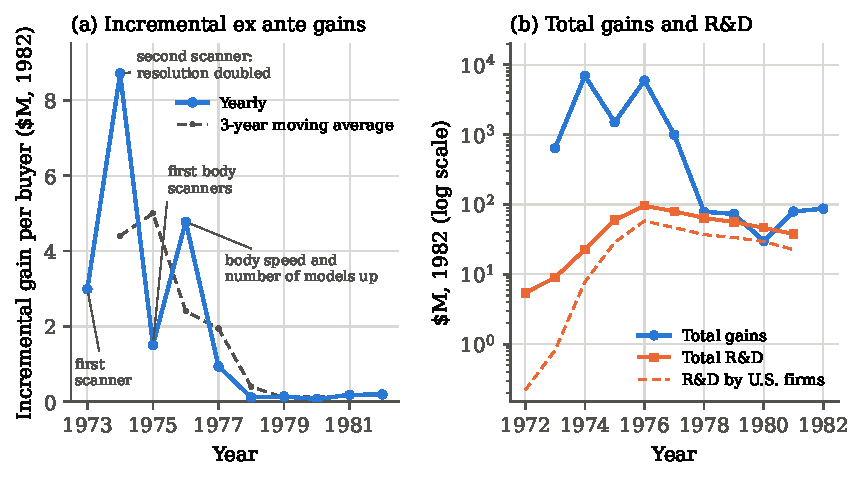
\includegraphics[width=\textwidth]{figures/ch10/trajtenberg_profile.pdf}
\caption{The time profile of the gains from innovation in CT scanners. Panel (a) shows the incremental ex ante gain per
buyer, with the 1973 value equal to the indirect estimate $\frac{K_0}{k}$, and its centered three-year moving average,
which is our computation. Panel (b) shows total gains $TW_t$ and research and development spending on a logarithmic
scale. The 1968--71 research total is a four-year aggregate and is omitted. Source: Trajtenberg (1985), Tables 9, 11
and 12.}
\label{fig:10-ct-profile}
\end{figure}

Second, the single largest gain came from the second scanner model, the EMI CT 1000 of 1974. Its design was almost
identical to the first EMI scanner, except that its resolution was almost doubled. The improvement transformed CT from a
demonstration of feasibility into a widely useful diagnostic tool (p.~78). Trajtenberg calls the early appearance of
such a big winner the ``Ford-T effect,'' after the Model T. Third, research spending tracked the level of activity in
the field with a one-year lead, but it was not closely related to the gains. The ratio of gains to research was about 80
to 1 for 1968--77, with research taken up to 1976. It was 1.4 for 1978--82, and in 1980 research spending exceeded the
benefits (p.~80).\footnote{The first ratio reproduces from Tables~11 and 12. Total gains of \$16,023.7 million in
1973--77 against total research of \$199.02 million in 1968--76 give 80.5. With the same one-year research lead and
no discounting, the two tables give $\frac{348.3}{284.40} = 1.22$ for 1978--82. The paper does not state the
definition behind its figure of 1.4 (our computation).}
Average returns are therefore a poor guide to policy. The question is less whether public support for research is
warranted than until when it should last. In CT, support was socially valuable in the early stages but not after 1976.
Trajtenberg notes that the British Department of Health supported the construction of the first prototype at EMI in
1970--72. An American neurologist, W.~H.~Oldendorf, had independently developed a similar device but could not pursue
it for lack of support (p.~80, n.~80). He presents the profile as evidence, from one case, that innovation can follow a
wave-like pattern.

\subsection{Robustness}\label{sec:10-ct-robustness}

Trajtenberg checks several of his choices, mostly in footnotes. The checks are scattered through the preceding
subsections, and we gather them here. The hedonic function was estimated in three forms, and Box-Cox comparisons
ranked the linear-log form first in half of the twelve cases (p.~37, n.~33). In the diffusion equation, a concave
ceiling gave very similar results to the linear one (pp.~67--68). The concave ceiling corresponds to exponentially
distributed reservation prices. Letting the incremental gains shift the speed of diffusion gave an effect that was
significant but very small (p.~68, n.~64). Repeat purchases are credited only with the incremental gain of their
year, so total gains are a lower bound in this respect (p.~70, n.~67). Adding profits of up to half of revenue to
the benefits would barely change the rate of return (p.~73). Returns to U.S. research and to total research serve
as upper and lower bounds on the true rate (pp.~71--72). Finally, the ex ante and ex post welfare measures are both
reported, and they differ by a factor of about seven (\cref{sec:10-ct-welfare}).

\subsection{Interpretation, critiques and contribution}\label{sec:10-ct-assessment}

Trajtenberg's study established that the magnitude of a product innovation can be measured by the consumer surplus it
creates, computed from an estimated discrete-choice model in characteristics space. Each step of the later literature
appears here in early form. Welfare comes from a log-sum surplus function. The nested logit is used to draw market
boundaries. Prices are related to characteristics through a hedonic function, and the per-buyer gains are linked to
diffusion and to research spending. \Citet{Petrin2002} builds on the template. \Citet[p.~238]{Bresnahan1997} writes
that Hausman takes on the question of the slope of $dd$ ``following Trajtenberg (1989).''

The limitations are of three kinds. The first concerns identification of price sensitivity. There are no instruments,
the residual-price coefficients have the wrong sign, and $\alpha$ is imported from another segment
(\cref{sec:10-ct-signal}). Because the money value of every gain divides by $\alpha$, the welfare numbers inherit this
uncertainty in full. The second concerns functional form. The MNL imposes IIA within branches, buyer heterogeneity is
absent after 1975, and the logit adds an entropy term for every new model (\cref{prop:10-clones,prop:10-entropy}). The
quadratic net utility extrapolates the value of large changes in characteristics. The estimated tastes change from year
to year, and the choice between ex ante and ex post measures changes the answer by a factor of seven. The second-stage
estimate of $\lambda$ carries little information about substitution between branches, as \eqref{eq:10-traj-lambda-implied} shows.
The third concerns interpretation. The buyers are hospitals, whose valuations may diverge from those of patients
(\cref{sec:10-ct-consumer}). The total gains rest on a reduced-form diffusion equation, and the value of the first scanner
is an indirect extrapolation from it.

These limitations do not overturn the qualitative conclusions. Early innovations in CT created large value relative
to their cost, gains concentrated in a few improvements, and returns to research fell sharply as the technology matured.
The precise numbers are less secure. The next case study, \citeauthor{Petrin2002}'s minivan, addresses several of the
weaknesses at once. It uses instruments for price, random coefficients disciplined by micro data, and a supply side
that lets rivals' prices respond. It also decomposes the welfare gain into the parts due to observed characteristics
and to the logit errors.
